\documentclass[11pt,a4paper]{article}

% ---------------------------------------------------------------
% Packages
% ---------------------------------------------------------------
\usepackage[utf8]{inputenc}
\usepackage[T1]{fontenc}
\usepackage{lmodern}
\usepackage[margin=1in]{geometry}
\usepackage{amsmath, amssymb, amsthm, mathtools}
\usepackage{graphicx}
\usepackage{booktabs}
\usepackage{multirow}
\usepackage{array}
\usepackage[expansion=false]{microtype}
\usepackage{listings}
\usepackage{xcolor}
\usepackage{textcomp}
\usepackage{enumitem}
\usepackage{tabularx}
\usepackage{hyperref}
\hypersetup{colorlinks=true, linkcolor=blue!50!black, citecolor=blue!50!black, urlcolor=blue!50!black}

\graphicspath{{heston_figures/}}
\setlength{\emergencystretch}{2em}

\lstdefinestyle{pystyle}{
    language=Python,
    basicstyle=\ttfamily\footnotesize,
    keywordstyle=\color{blue},
    commentstyle=\color{gray},
    stringstyle=\color{teal},
    showstringspaces=false,
    breaklines=true,
    frame=single,
    tabsize=4
}

% ---------------------------------------------------------------
% Theorem environments and macros
% ---------------------------------------------------------------
\theoremstyle{plain}
\newtheorem{theorem}{Theorem}[section]
\newtheorem{proposition}[theorem]{Proposition}
\newtheorem{lemma}[theorem]{Lemma}
\theoremstyle{definition}
\newtheorem{definition}[theorem]{Definition}
\newtheorem{remark}[theorem]{Remark}

\newcommand{\dd}{\mathrm{d}}
\newcommand{\E}{\mathbb{E}}
\newcommand{\Q}{\mathbb{Q}}
\newcommand{\R}{\mathbb{R}}
\newcommand{\Var}{\operatorname{Var}}
\newcommand{\Real}{\operatorname{Re}}
\newcommand{\ind}{\mathbf{1}}
\newcommand{\iu}{\mathrm{i}}
\DeclareMathOperator*{\argmin}{arg\,min}

\title{\textbf{Calibration of the Heston Stochastic Volatility Model:\\
Theoretical Framework, Numerical Methods, and Limitations}}
\author{\textbf{Elias Benguedda}}
\date{October 2026}

\begin{document}

\maketitle

\begin{abstract}
This paper presents a calibration of the Heston (1993) stochastic volatility model to European option quotes, applied to a CAC40 option chain. We review the model dynamics and the main properties of the Cox--Ingersoll--Ross (CIR) variance process, derive the characteristic function from the affine Riccati system, and obtain semi-analytical prices by Gil--Pelaez inversion. We then analyse the inverse problem: loss functions, first-order equivalence between price and implied-volatility losses, identifiability, regularization and optimization strategy.

We document a full Python implementation. The forward curve is rebuilt from put-call parity and a piecewise-constant borrow-plus-dividend curve is bootstrapped from it. The model reproduces the market surface with an implied volatility RMSE of $0.42$ volatility points. A time-dependent extension with piecewise constant $\theta$, $\xi$ and $\rho$ lowers it to $0.12$--$0.15$; out-of-sample and noise tests show that a time-dependent $\theta$ alone is a robust improvement, whereas the fully time-dependent parameters are not identified by a single day of vanilla quotes. Finally, we discuss numerical stability issues, parameter identification challenges and the structural limitations of the model. This paper is linked to my GitHub, which can be found on my portfolio\footnote{\url{https://portfolio-eliasbenguedda.fr}}, and all scripts are available in the same repository.
\end{abstract}

\clearpage

\tableofcontents
\newpage

% ===============================================================
\section{Introduction}
\label{sec:intro}
% ===============================================================

\subsection{Motivation}
The Black--Scholes framework~\cite{blackscholes} assumes a constant volatility, and therefore predicts a flat implied volatility surface across all strikes and maturities. As we know, this assumption is too simple and does not permit to explain the volatility behavior. Implied volatility is typically a decreasing function of strike\footnote{This is the skew.}, with a term structure that depends on maturity. We are then working on a 3 dimensions problem. To capture these market phenomena, stochastic volatility models let the variance of the underlying follow its own diffusion process.

The Heston model~\cite{heston1993} remains one of the most widely used stochastic volatility models in quantitative finance. Its primary advantage lies in the existence of a semi-closed-form solution for European options using Fourier transform techniques as we will see later in this paper, which allows computationally efficient calibration against market option quotes.

Beyond the model dynamics themselves, a calibration exercise on real market data exposes a second, often underestimated, layer of complexity: the market does not directly quote the risk-neutral forward price of the underlying. Interest-rate and dividend assumptions must be inferred from the option prices themselves any calibration. Section~\ref{sec:forward} is dedicated to this problem.



\subsection{Organization of the paper}
Section~\ref{sec:prelim} fixes notation and recalls market preliminaries. Section~\ref{sec:heston} presents the model and the properties of the variance process. Section~\ref{sec:data} describes the data. Section~\ref{sec:pricing} derives the pricing formulas. Section~\ref{sec:forward} builds the forward and dividend curve. Section~\ref{sec:calibration} describes the implementation and the calibration methodology. Section~\ref{sec:results} reports the empirical results. Section~\ref{sec:td} extends the model to time-dependent parameters and tests the extension for overfitting. Section~\ref{sec:limits} discusses limitations, Section~\ref{sec:next-steps} lists next steps, and Section~\ref{sec:conclusion} concludes. Appendix~\ref{app:code} gives excerpts of the Python implementation.





\clearpage
% ===============================================================
\section{Market Preliminaries and Notation}
\label{sec:prelim}
% ===============================================================

\subsection{Forward, discounting and put-call parity}
Let $S_0$ denote the spot price, $r(t)$ the continuously compounded zero-coupon rate for maturity $t$ and $q(t)$ the instantaneous cost of carry (dividends plus repo/borrow spread). Define the discount factor and the forward price
\begin{equation}
    D(t) = e^{-r(t)t}, \qquad F(t) = S_0\, \exp\Bigl(r(t)t-\int_0^t q(s)\,\dd s\Bigr),
    \label{eq:forward}
\end{equation}
Under the risk-neutral measure $\Q$, $\E^{\Q}[S_T]=F(T)$. European call and put prices are
\begin{equation}
    C(K,T) = D(T)\,\E^{\Q}\bigl[(S_T-K)^+\bigr], \qquad
    P(K,T) = D(T)\,\E^{\Q}\bigl[(K-S_T)^+\bigr].
\end{equation}
Since $(S_T-K)^+-(K-S_T)^+=S_T-K$, taking expectations gives the put-call parity relation
\begin{equation}
    C(K,T)-P(K,T) = D(T)\bigl(F(T)-K\bigr).
    \label{eq:pcp}
\end{equation}
Because the put-call parity does not depend on the model, it is therefore the tool used in Section~\ref{sec:forward} to recover $F(t)$ from market quotes.





\subsection{Static no-arbitrage constraints}
A quoted surface $(K,t)\mapsto C(K,t)$ is free of static arbitrage if and only if the following conditions are respected (see e.g.~\cite{gatheral, gatheraljacquier}):
\begin{align}
    &\text{(monotonicity)} && -D(t) \le \frac{\partial C}{\partial K}(K,t) \le 0, \label{eq:mono}\\
    &\text{(butterfly)} && \frac{\partial^2 C}{\partial K^2}(K,t) \ge 0, \label{eq:butterfly}\\
    &\text{(calendar)} && t\mapsto \frac{C(F(t)e^{k},t)}{D(t)F(t)} \text{ is non-decreasing for fixed } k. \label{eq:calendar}
\end{align}
By the Breeden--Litzenberger identity~\cite{breeden}, $\partial^2C/\partial K^2 = D(t)\,f_{S_t}(K)$ where $f_{S_t}$ is the risk-neutral density of $S_t$, so~\eqref{eq:butterfly} says that this density is non-negative. Note that the calendar condition~\eqref{eq:calendar} is expressed in forward-normalized form and therefore requires the forward curve $F(t)$ to be known. Heston prices are arbitrage-free by construction.







\subsection{Notation}
Table~\ref{tab:notation} in Appendix~\ref{app:notation} summarizes the notation used throughout the paper.







\clearpage
% ===============================================================
\section{The Heston Model}
\label{sec:heston}
% ===============================================================

\subsection{Dynamics}
Under the risk-neutral pricing measure $\Q$, the asset price process $S_t$ and its variance process $v_t$ follow the coupled stochastic differential equations (SDEs)
\begin{align}
    \dd S_t &= (r - q) S_t \,\dd t + \sqrt{v_t}\, S_t \,\dd W_t^S, \label{eq:sde-S}\\
    \dd v_t &= \kappa (\theta - v_t)\,\dd t + \xi \sqrt{v_t}\,\dd W_t^v, \label{eq:sde-v}
\end{align}
with correlated standard Brownian motions
\begin{equation}
    \dd\langle W^S, W^v \rangle_t = \rho\,\dd t, \qquad \rho \in [-1, 1].
    \label{eq:corr}
\end{equation}

Here $r$ denotes the risk-free (zero-coupon) rate and $q$ the continuously compounded cost of carry, encompassing both the dividend yield and the repo/borrow spread of the underlying. Both $r$ and $q$ are, in practice, term structures rather than constants. Since they are deterministic, they only enter the model through the forward $F(t)$ of~\eqref{eq:forward}: in the implementation the drift of $S$ is taken from the implied forward curve, so that $\E^\Q[S_T]=F(T)$ holds exactly at every maturity. The $\Q$-dynamics~\eqref{eq:sde-v} implicitly absorbs the market price of variance risk into the parameters $(\kappa,\theta)$.

Applying It\^o's formula to $x_t=\ln S_t$ gives the log-price dynamics
\begin{equation}
    \dd x_t = \Bigl(r - q - \tfrac12 v_t\Bigr)\dd t + \sqrt{v_t}\,\dd W_t^S,
    \label{eq:sde-x}
\end{equation}
which is the form used to derive the characteristic function in Section~\ref{sec:pricing}.

\subsection{Parameter definitions}
The model is governed by five parameters $\Theta = (v_0, \kappa, \theta, \xi, \rho)$:
\begin{itemize}
    \item $v_0 > 0$: instantaneous variance at $t=0$;
    \item $\theta > 0$: long-term mean variance;
    \item $\kappa > 0$: rate of mean reversion;
    \item $\xi > 0$: volatility of volatility (vol-of-vol);
    \item $\rho \in [-1, 1]$: correlation coefficient between spot and variance returns. A negative $\rho$ accounts for the leverage effect observed in equity markets.
\end{itemize}
The aim of the calibration is to find the vector $\Theta$ that minimizes the error between the market and the model over all the quoted points of the volatility surface.

\subsection{The pricing PDE}
Let $V(t,S,v)$ be the value of a European derivative. By the Feynman--Kac theorem, $V$ solves the following PDE:
\begin{equation}
    \frac{\partial V}{\partial t} + \tfrac12 v S^2\frac{\partial^2 V}{\partial S^2}
    + \rho\xi v S\frac{\partial^2 V}{\partial S\,\partial v}
    + \tfrac12\xi^2 v\frac{\partial^2 V}{\partial v^2}
    + (r-q)S\frac{\partial V}{\partial S}
    + \kappa(\theta-v)\frac{\partial V}{\partial v}
    - rV = 0,
    \label{eq:hestonpde}
\end{equation}
with terminal condition $V(T,S,v)=(S-K)^+$ for a call. Contrary to Black--Scholes, no closed form in terms of elementary functions exists; the solution is obtained by Fourier methods (Section~\ref{sec:pricing})\footnote{ The mixed-derivative term $\rho\xi vS\,\partial_{S}\partial_{v}V$ is what allows the model to generate skew.}.

\subsection{Properties of the variance process}
The variance~\eqref{eq:sde-v} is a CIR process~\cite{cir}. We will use the following properties.
For $t>s$ and $\tau=t-s$, conditionally on $v_s$,
\begin{equation}
    v_t \overset{d}{=} c(\tau)\,\chi'^2_{\delta}\bigl(\lambda(\tau)\bigr), \quad
    c(\tau)=\frac{\xi^2\bigl(1-e^{-\kappa\tau}\bigr)}{4\kappa},\quad
    \delta=\frac{4\kappa\theta}{\xi^2},\quad
    \lambda(\tau)=\frac{4\kappa e^{-\kappa\tau}}{\xi^2\bigl(1-e^{-\kappa\tau}\bigr)}\,v_s,
    \label{eq:cir-transition}
\end{equation}
where $\chi'^2_\delta(\lambda)$ denotes a non-central chi-squared random variable with $\delta$ degrees of freedom and non-centrality $\lambda$.
Taking expectations in~\eqref{eq:sde-v} gives $\frac{\dd}{\dd t}\E[v_t]=\kappa(\theta-\E[v_t])$, hence
\begin{equation}
    \E[v_t] = \theta + (v_0-\theta)e^{-\kappa t}.
    \label{eq:mean-v}
\end{equation}
Applying It\^o's formula to $v_t^2$ and solving the resulting linear ODE for $\E[v_t^2]$ yields
\begin{equation}
    \Var(v_t) = \frac{v_0\,\xi^2}{\kappa}\bigl(e^{-\kappa t}-e^{-2\kappa t}\bigr)
    + \frac{\theta\,\xi^2}{2\kappa}\bigl(1-e^{-\kappa t}\bigr)^2.
    \label{eq:var-v}
\end{equation}
For small $t$, $\Var(v_t)\approx \xi^2 v_0\, t$, as expected from the diffusion coefficient at $t=0$.

\subsection{The Feller condition}


As $t\to\infty$, $v_t$ converges in law to a Gamma distribution\footnote{\url{https://en.wikipedia.org/wiki/Gamma_distribution}} with shape $\alpha=2\kappa\theta/\xi^2$ and rate $\beta=2\kappa/\xi^2$, whose mean $\alpha/\beta=\theta$ and variance $\alpha/\beta^2=\theta\xi^2/(2\kappa)$ are consistent with~\eqref{eq:mean-v}--\eqref{eq:var-v}. Since the Gamma density behaves like $v^{\alpha-1}$ near zero, the stationary density blows up at zero when $\alpha<1$.
To prevent the variance process $v_t$ from reaching zero, the parameters must satisfy
\begin{equation}
    2 \kappa \theta > \xi^2.
    \label{eq:feller}
\end{equation}
When this condition holds, the zero boundary is not attainable, which ensures strict positivity of $v_t$. The Feller ratio $2\kappa\theta/\xi^2$ is thus precisely the shape parameter of the stationary Gamma law. In practice, market calibrations often violate this condition (ours gives a ratio of $0.49$, Section), requiring appropriate boundary treatment in Monte Carlo algorithms (absorption, reflection or full truncation). Violating~\eqref{eq:feller} is not an issue for Fourier pricing, since the characteristic function remains valid.


\paragraph{Integrated variance.} Integrating~\eqref{eq:mean-v} over $[0,T]$,
\begin{equation}
    \E\!\left[\int_0^T v_t\,\dd t\right] = \theta T + (v_0-\theta)\,\frac{1-e^{-\kappa T}}{\kappa}.
    \label{eq:int-var}
\end{equation}
Since the total variance of the log-price is, to leading order, $\int_0^Tv_t\,\dd t$, the at-the-money implied variance is approximately $w(T)/T$ with $w(T)$ the right-hand side of~\eqref{eq:int-var}: the ATM term structure is governed by $(v_0,\theta,\kappa)$, interpolating between $v_0$ at short maturity and $\theta$ at long maturity with time-scale $1/\kappa$.

\subsection{Skew and effect of the parameters}
For small maturities, the ATM skew of Heston admits a finite limit,
\begin{equation}
    \lim_{T\to0}\frac{\partial\sigma_{\mathrm{BS}}}{\partial k}\bigg|_{k=0} = \frac{\rho\,\xi}{4\sqrt{v_0}},
    \label{eq:smallskew}
\end{equation}
where $k=\ln(K/F)$. (This is the classical small-time asymptotics for one-factor stochastic volatility models; see~\cite{gatheral}.) Two consequences are important for calibration: (i) the skew is proportional to $\rho\xi$, so that $\rho$ and $\xi$ are not separately identified by the first-order slope, only by higher-order (curvature) information; (ii) for equity indices with $\rho<0$, the skew is negative, as observed. Table~\ref{tab:params} summarizes the qualitative effect of each parameter on the surface.

\begin{table}[h]
\centering
\begin{tabular}{@{}p{1.8cm}p{5.2cm}p{7.0cm}@{}}
\toprule
Parameter & Effect on the smile & Effect on the term structure \\
\midrule
$v_0$ & Vertical level of short-dated smile & Short-maturity ATM level $\approx\sqrt{v_0}$ \\
$\theta$ & Vertical level of long-dated smile & Long-maturity ATM level $\approx\sqrt{\theta}$ \\
$\kappa$ & Speed at which the smile flattens with maturity & Time scale $1/\kappa$ of the transition $v_0\to\theta$ \\
$\xi$ & Curvature (convexity) of the smile; lifts the wings & Amplifies skew and curvature at short/mid maturities \\
$\rho$ & Skew (negative $\rho$: downward-sloping smile) & Skew decays with maturity at a rate governed by $\kappa$ \\
\bottomrule
\end{tabular}
\caption{Qualitative effect of the Heston parameters on the implied volatility surface.}
\label{tab:params}
\end{table}

\clearpage
% ===============================================================
\section{Data}
\label{sec:data}
% ===============================================================

The data come from a public GitHub repository~\cite{data}; we do not investigate data quality issues beyond the filters described below. The valuation date is 12 February 2025, with a CAC40 spot $S_0=8042.19$.

\subsection{Rates} For the discounting, we use the EURIBOR 6M zero-coupon curve, given at 15 pillars from $0.02$ to $5$ years. The zero rates are interpolated with a Piecewise Cubic Hermite Interpolating Polynomial (PCHIP interpolator)~\cite{fritsch} (monotone, without overshoot) and extrapolated beyond the last pillar\footnote{This type of interpolation will be studied in the yield curve document in my portfolio.}. Over the maturities of the option chain the zero rate decreases from $2.68\%$ at 9 days to $2.25\%$ at two years, then rises slightly to $2.30\%$ at five years (Figure~\ref{fig:euribor}).

\begin{figure}[htbp]
    \centering
    \includegraphics[width=0.75\textwidth]{EURIBOR6M_curve.png}
    \caption{EURIBOR 6M zero-coupon curve, PCHIP interpolation.}
    \label{fig:euribor}
\end{figure}

\subsection{Options} The option chain contains 142 strikes over 13 expiries, with both a call and a put price for each strike: 11 strikes per expiry, except 10 for the last one. Expiries are only listed by month and year (from February 2025 to December 2029); we assume that the options expire on the third Friday of the month and measure time to expiry in years with the ACT/365 convention. This gives maturities from $9$ days ($T=0.0247$) to $4.86$ years ($T=4.8575$). The strike range widens with maturity, from $7925$--$8200$ at 9 days to $5600$--$11200$ at 4 years.

Only out-of-the-money (OTM) options are used for the volatility surface, because OTM options are usually the most liquid, and their prices are the most sensitive to volatility relative to their level. All 142 OTM quotes have a Black implied volatility, so no quote is discarded.




\clearpage
% ===============================================================
\section{Semi-Analytical Option Pricing via Fourier Inversion}
\label{sec:pricing}
% ===============================================================

The European call price $C(S_0, K, T)$ with strike $K$ and maturity $T$ can be written as
\begin{equation}
    C(S_0, K, T) = S_0 e^{-q T} P_1 - K e^{-r T} P_2 = D(T)\bigl(F(T)P_1-KP_2\bigr),
    \label{eq:call-P1P2}
\end{equation}
where $P_2=\Q(S_T>K)$ and $P_1=\E^{\Q}[S_T\ind_{\{S_T>K\}}]/F(T)$ is the exercise probability under the share measure. Both are evaluated via Fourier inversion of the characteristic function $\phi(u; T)$.

\subsection{Characteristic function via the Riccati system}
Using the log-price $x_t = \ln S_t$, the characteristic function is $\phi(u;T) = \E^{\Q}\bigl[ e^{\iu u x_T} \mid x_0, v_0 \bigr]$.


For $u\in\R$ (and by analytic continuation for admissible complex $u$),
\begin{equation}
    \phi(u; T) = \exp\Bigl( C(u, T)\theta + D(u, T) v_0 + \iu u \bigl( \ln S_0 + (r - q) T \bigr) \Bigr),
    \label{eq:cf}
\end{equation}
where $C(u,T)$ and $D(u,T)$ follow Gatheral's~\cite{gatheral} numerically stable formulation
\begin{align}
    D(u, T) &= \frac{\kappa - \iu \rho \xi u - d}{\xi^2} \left( \frac{1 - e^{-d T}}{1 - g e^{-d T}} \right), \label{eq:D}\\
    C(u, T) &= \frac{\kappa}{\xi^2} \left[ (\kappa - \iu \rho \xi u - d) T - 2 \ln \left( \frac{1 - g e^{-d T}}{1 - g} \right) \right], \label{eq:C}
\end{align}
with
\begin{align}
    d &= \sqrt{(\kappa - \iu \rho \xi u)^2 + \xi^2 (u^2 + \iu u)}, \label{eq:d}\\
    g &= \frac{\kappa - \iu \rho \xi u - d}{\kappa - \iu \rho \xi u + d}. \label{eq:g}
\end{align}



\begin{remark}[Term structures and forward normalization]\label{rem:fwd-cf}
With deterministic $r(t)$ and $q(t)$, only changes: $\iu u(r-q)\tau$ becomes $\iu u\int_0^T(r-q)\,\dd t=\iu u\ln\bigl(F(T)/S_0\bigr)$. It is therefore convenient to work with the forward log-moneyness of the terminal price, $X_T=\ln\bigl(S_T/F(T)\bigr)$, whose characteristic function
\begin{equation}
    \phi_X(u;T)=\E^\Q\bigl[e^{\iu uX_T}\bigr]=\exp\bigl(C(u,T)\theta+D(u,T)v_0\bigr)
    \label{eq:cf-fwd}
\end{equation}
does not depend on rates or dividends at all. The martingale condition reads $\phi_X(-\iu;T)=\E^\Q[S_T]/F(T)=1$; indeed $u=-\iu$ gives $u^2+\iu u=0$, hence $d=b$, $C=D=0$. The implementation (\texttt{HestonModel.characteristic\_function}) uses~\eqref{eq:cf-fwd}, and all market inputs enter the price only through $F(T)$ and $D(T)$.
\end{remark}


\subsection{Probabilities via Gil--Pelaez inversion}
By the Gil--Pelaez inversion theorem~\cite{gilpelaez}, the distribution function of a random variable $X$ with characteristic function $\varphi_X$ satisfies
\begin{equation}
    \Q(X>x)=\frac12+\frac1\pi\int_0^\infty\Real\!\left[\frac{e^{-\iu ux}\varphi_X(u)}{\iu u}\right]\dd u.
\end{equation}
Applied to $X=x_T=\ln S_T$ under $\Q$ (characteristic function $\phi$) and under the share measure (characteristic function $\phi_1(u)=\E^{\Q}[S_Te^{\iu ux_T}]/F=\phi(u-\iu)/\phi(-\iu)$, with $\phi(-\iu)=\E^\Q[S_T]=F(T)$), we obtain
\begin{align}
    P_2 &= \frac12+\frac1\pi\int_0^\infty\Real\!\left[\frac{e^{-\iu u\ln K}\,\phi(u;T)}{\iu u}\right]\dd u,\label{eq:P2}\\
    P_1 &= \frac12+\frac1\pi\int_0^\infty\Real\!\left[\frac{e^{-\iu u\ln K}\,\phi(u-\iu;T)}{\iu u\,F(T)}\right]\dd u.\label{eq:P1}
\end{align}
Both integrands are bounded near $u=0$: since $\phi(0)=1$, the real part of $e^{-\iu u\ln K}\phi(u)/(\iu u)$ converges to $\E[x_T]-\ln K$ as $u\to0$. Injecting~\eqref{eq:P1}--\eqref{eq:P2} in~\eqref{eq:call-P1P2} gives the Heston call price; the put price follows from parity~\eqref{eq:pcp}. This representation requires two integrals per price, each with an integrand that decays only like $1/u$ times the characteristic function.

\subsection{The Lewis single-integral formula (implemented)}
Lewis (2001)~\cite{lewis} obtains the call price with a single integral by moving the Fourier inversion to the line $\operatorname{Im} z=\frac12$, where both the characteristic function and the transform of the payoff are analytic. With $X_T=\ln(S_T/F(T))$ and $k=\ln\bigl(F(T)/K\bigr)$,
\begin{equation}
    C(K,T)=D(T)\left[F(T)-\frac{\sqrt{F(T)K}}{\pi}\int_0^\infty\Real\Bigl[e^{\iu uk}\,\phi_X\bigl(u-\tfrac{\iu}{2};T\bigr)\Bigr]\frac{\dd u}{u^2+\frac14}\right].
    \label{eq:lewis}
\end{equation}
The first term $D(T)F(T)$ is the residue picked up when the contour crosses the pole of the payoff transform at $z=\iu$. Compared with~\eqref{eq:P2}--\eqref{eq:P1}, the formula needs a single evaluation of $\phi_X$ per node, its integrand is bounded at $u=0$ and decays at least like $u^{-2}$, and the characteristic function does not depend on the strike. The integral can therefore be computed once on a fixed grid of $u$ and reused for all the strikes of a maturity.

\paragraph{Implementation.} \texttt{HestonModel.price\_vanillas} evaluates the equation~\eqref{eq:lewis} for all the strikes of one maturity in a single vectorized call: $\phi_X(u-\iu/2)$ is computed on a uniform grid of $4000$ points on $[10^{-8},1000]$, and the integral is computed with the trapezoidal rule. Puts are obtained by put-call parity. Doubling the grid resolution and extending it to $u_{\max}=4000$ changes the prices of the 142 quotes by less than $\text{\texteuro}0.06$ at the retained parameters, for the shortest ($T=0.0247$), a middle ($T=1.10$) and the longest ($T=4.86$) expiry alike. This is well below the calibration error of Section~\ref{sec:results}.

\subsection{Carr--Madan FFT pricing}
Following Carr and Madan (1999)~\cite{carrmadan}, let $k=\ln K$ be the log-strike, $\alpha>0$ a damping factor and $c_T(k)=e^{\alpha k}C(k,T)$ the modified call price, which is square-integrable in $k$ provided $\E^\Q[S_T^{\alpha+1}]<\infty$. Its Fourier transform is $\psi_T(v)=\int_{-\infty}^{\infty}e^{\iu vk}c_T(k)\,\dd k$ with
\begin{equation}
    \psi_T(v) = \frac{e^{-rT}\,\phi\bigl(v-(\alpha+1)\iu;T\bigr)}{\alpha^2+\alpha-v^2+\iu(2\alpha+1)v},
\end{equation}
and Fourier inversion gives
\begin{equation}
    C(K, T) = \frac{e^{-\alpha k-rT}}{\pi} \Real\int_0^\infty e^{-\iu vk}\, \frac{\phi(v - (\alpha + 1)\iu; T)}{\alpha^2 + \alpha - v^2 + \iu(2\alpha + 1)v} \, \dd v.
    \label{eq:carrmadan}
\end{equation}
Discretizing with $N$ points, step $\eta$ in $v$ and step $\lambda$ in $k$, subject to the FFT constraint $\lambda\eta=2\pi/N$, and setting $v_j=\eta(j-1)$, $k_m=-b+\lambda(m-1)$ with $b=N\lambda/2$, we obtain
\begin{equation}
    C(k_m,T)\approx\frac{e^{-\alpha k_m}}{\pi}\sum_{j=1}^{N}e^{-\iu\frac{2\pi}{N}(j-1)(m-1)}\,e^{\iu bv_j}\,\psi_T(v_j)\,\frac{\eta}{3}\bigl(3+(-1)^j-\delta_{j-1}\bigr),
\end{equation}
where the Simpson-rule weights $\frac{\eta}{3}(3+(-1)^j-\delta_{j-1})$ improve accuracy. A single FFT of size $N$ thus prices the whole grid of $N$ strikes in $\mathcal O(N\log N)$ operations. The accuracy is controlled by the trade-off between $\eta$ (integration accuracy) and $\lambda=2\pi/(N\eta)$ (strike resolution), and by the choice of $\alpha$. With only 11 strikes per maturity in our data, the vectorized Lewis quadrature is already fast enough, and the FFT is left as a future optimization (Section~\ref{sec:next-steps}).

\subsection{The COS method}
The COS method of Fang and Oosterlee~\cite{fangoosterlee} expands the density of $y_T=\ln(S_T/K)$ on a truncated interval $[a,b]$ in a cosine series whose coefficients are given by the characteristic function, and prices a call as
\begin{equation}
    C(K,T)\approx e^{-rT}\sum_{k=0}^{N-1}{}^{\prime}\ \Real\Bigl[e^{-\iu\omega_k\ln K}\,\phi(\omega_k;T)\,e^{-\iu\omega_ka}\Bigr]V_k,\qquad \omega_k=\frac{k\pi}{b-a},
\end{equation}
where $\sum'$ halves the first term. The payoff coefficients of a call are
\begin{equation}
    V_k=\frac{2}{b-a}\,K\bigl(\chi_k(0,b)-\psi_k(0,b)\bigr),
\end{equation}
with
\begin{align}
    \chi_k(c,d)&=\frac{1}{1+\omega_k^2}\Bigl[\cos\bigl(\omega_k(d-a)\bigr)e^{d}-\cos\bigl(\omega_k(c-a)\bigr)e^{c}\nonumber\\
    &\qquad\qquad+\omega_k\sin\bigl(\omega_k(d-a)\bigr)e^{d}-\omega_k\sin\bigl(\omega_k(c-a)\bigr)e^{c}\Bigr],\\
    \psi_k(c,d)&=\begin{cases}\dfrac{\sin(\omega_k(d-a))-\sin(\omega_k(c-a))}{\omega_k}, & k\ge1,\\[2mm] d-c, & k=0.\end{cases}
\end{align}
The truncation interval is chosen as $[a,b]=[c_1-L\sqrt{c_2+\sqrt{c_4}},\,c_1+L\sqrt{c_2+\sqrt{c_4}}]$ with $L\approx10$, where $c_n$ are the cumulants of $y_T$ obtained by differentiating $\ln\phi$ at zero. Because the series converges exponentially in $N$ for smooth densities, a few dozen terms often suffice, which makes COS the natural candidate for the inner pricing loop of a calibration.

\subsection{Greeks and risk-neutral density}
Since $C(S_0,K)$ is positively homogeneous of degree one in $(S_0,K)$ (because $S_T/S_0$ has a law which does not depend on $S_0$), Euler's relation gives $C=S_0\partial_{S_0}C+K\partial_KC$. As $\partial_KC=-e^{-rT}P_2$, we obtain the Delta in closed form
\begin{equation}
    \Delta=\frac{\partial C}{\partial S_0}=\frac{C+Ke^{-rT}P_2}{S_0}=e^{-qT}P_1.
    \label{eq:delta}
\end{equation}
The risk-neutral density of $\ln S_T$ is
\begin{equation*}
    f_{x_T}(x)=\frac1\pi\int_0^\infty\Real\bigl[e^{-\iu ux}\phi(u;T)\bigr]\dd u,
\end{equation*}
hence $\partial_K^2C=e^{-rT}f_{S_T}(K)=e^{-rT}f_{x_T}(\ln K)/K$, and by homogeneity the Gamma is
\begin{equation}
    \Gamma=\frac{\partial^2C}{\partial S_0^2}=\frac{K^2}{S_0^2}\,\frac{\partial^2C}{\partial K^2}.
\end{equation}
Sensitivities with respect to the model parameters are obtained by differentiating under the integral sign. Because $\phi$ depends on $v_0$ through $e^{D(u,T)v_0}$, we have $\partial_{v_0}\phi(u)=D(u,T)\phi(u)$, so that
\begin{align}
    \frac{\partial P_2}{\partial v_0}&=\frac1\pi\int_0^\infty\Real\!\left[\frac{e^{-\iu u\ln K}D(u,T)\phi(u;T)}{\iu u}\right]\dd u,\\
    \frac{\partial P_1}{\partial v_0}&=\frac1\pi\int_0^\infty\Real\!\left[\frac{e^{-\iu u\ln K}D(u-\iu,T)\phi(u-\iu;T)}{\iu u\,F(T)}\right]\dd u,
\end{align}
and $\partial_{v_0}C=S_0e^{-qT}\partial_{v_0}P_1-Ke^{-rT}\partial_{v_0}P_2$. Analogous formulas hold for $\kappa,\theta,\xi,\rho$ and provide analytical gradients for the calibration (see~\cite{cui}). They are not implemented yet: the optimizers of Section~\ref{sec:calibration} use finite-difference gradients.

\clearpage
% ===============================================================
\section{The Forward and Dividend Curve}
\label{sec:forward}
% ===============================================================

\subsection{Motivation}
Equity index options are quoted against a forward price $F(t)$ that is not directly observable. The rate $r(t)$ can be taken from a liquid interest rate curve (here the EURIBOR 6M zero-coupon curve), but the effective cost of carry $q(t)$, combining dividends and repo/borrow, has to be calculated. For equity indices it is markedly seasonal, concentrated around the dividend-payment window (April--June for the CAC40).

\subsection{Effect of a mis-specified forward}

On our data, the bootstrapped carry of Section~\ref{sec:bootstrap} integrates to $\int_0^Tq(t)\,\dd t=0.136$ at the longest maturity $T=4.86$, i.e. an average carry of $2.8\%$ per year. Setting $\hat q=0$ therefore overstates the 5-year forward by $e^{0.136}-1\approx14.6\%$: $\hat F=8992$ instead of $F=7847$. This is the textbook signature of an overstated forward: calls overpriced, puts underpriced, with a distortion that grows with $T$.

The bias is not only a vertical price shift. In forward log-moneyness $k=\ln(K/F)$, using $\hat F$ instead of $F$ shifts the strike axis by
\begin{equation}
    \hat k=\ln\frac{K}{\hat F}=k-\int_0^T\bigl(q(t)-\hat q(t)\bigr)\,\dd t,
\end{equation}
But then the whole smile is translated horizontally. Here the shift is $0.136$ at $T=4.86$; with a long-dated ATM volatility of about $17\%$, the total standard deviation is $\sigma\sqrt T\approx0.37$, so the shift is more than a third of a standard deviation, which is large compared with typical smile widths.

\subsection{Implied forward via put-call parity}
For a fixed expiry $T$, put-call parity~\eqref{eq:pcp} implies that the call and put price curves, as functions of strike, intersect exactly at the ATM-forward strike $K = F(T)$:
\begin{equation}
    C(F(T), T) = P(F(T), T).
    \label{eq:atmforward}
\end{equation}
Given a discrete set of listed strikes $K_1 < \dots < K_n$, we compute the call–put differences $d_i = C(K_i,T) - P(K_i,T)$ and interpolate them linearly between consecutive strikes. By put–call parity, $C(K,T) - P(K,T) = D(T)(F(T) - K)$, which is strictly decreasing and affine in $K$ with slope $-D(T)$. Hence $F(T)$ is its unique root, and it lies on the segment $[K_i, K_{i+1}]$ where $d_i$ changes sign. On this segment, the root of the linear interpolant is given in closed form by
$$F(T) = K_i - d_i\frac{K_{i+1} - K_i}{d_{i+1} - d_i}.$$
If the listed strikes do not bracket the forward, so that no sign change occurs, we extrapolate linearly from the first segment when all $d_i < 0$ and from the last segment when all $d_i > 0$. This is consistent with the affine form implied by parity.

Table~\ref{tab:forwards} gives the implied forwards. They drop by $136$ points between the April and June 2025 expiries and by $108$ points between March and June 2026, which is the ex-dividend season of the CAC40 constituents.

\begin{table}[htbp]
\centering
\small
\begin{tabular}{@{}lrrrlrrr@{}}
\toprule
Expiry & $T$ & $F(T)$ & $q_k$ (\%) & Expiry & $T$ & $F(T)$ & $q_k$ (\%) \\
\midrule
Feb 2025 & 0.0247 & 8049.0 & $-0.75$ & Jun 2026 & 1.3479 & 7930.9 & 7.54 \\
Mar 2025 & 0.1014 & 8066.5 & $-0.16$ & Sep 2026 & 1.5973 & 7943.9 & 1.52 \\
Apr 2025 & 0.1781 & 8079.0 & 0.62 & Dec 2026 & 1.8466 & 7969.9 & 0.87 \\
Jun 2025 & 0.3507 & 7943.5 & 12.33 & Dec 2027 & 2.8438 & 7897.7 & 3.19 \\
Sep 2025 & 0.6000 & 7987.5 & 0.05 & Dec 2028 & 3.8411 & 7872.8 & 2.65 \\
Dec 2025 & 0.8493 & 8003.0 & 1.36 & Dec 2029 & 4.8575 & 7847.3 & 2.69 \\
Mar 2026 & 1.0986 & 8039.1 & 0.32 & & & & \\
\bottomrule
\end{tabular}
\caption{Implied forwards from put-call parity ($S_0=8042.19$) and bootstrapped borrow-plus-dividend yield $q_k$ on $(T_{k-1},T_k]$.}
\label{tab:forwards}
\end{table}

\clearpage
\subsection{Dividend bootstrap}
\label{sec:bootstrap}
Assuming the instantaneous borrow-plus-dividend yield $q(t)$ is piecewise constant between consecutive listed expiries $T_1 < T_2 < \dots < T_n$, the forward at $T_k$ satisfies
\begin{equation}
    F(T_k) = S_0 \exp\left( r(T_k) T_k - \sum_{j=1}^{k} q_j (T_j - T_{j-1}) \right), \qquad T_0 := 0,
    \label{eq:F-bootstrap}
\end{equation}
which is solved recursively for each piecewise-constant segment $q_k$:
\begin{equation}
    q_k = \frac{1}{T_k - T_{k-1}} \ln \left( \frac{S_0 \exp\left(r(T_k)T_k - \sum_{j=1}^{k-1} q_j(T_j - T_{j-1})\right)}{F(T_k)} \right).
    \label{eq:qk}
\end{equation}
The resulting step function $q(t)$ is extrapolated flat after $T_n$ (on $[0,T_1]$ it equals $q_1$). The forward at an arbitrary maturity $T$ is then recovered as
\begin{equation}
    F(T) = S_0 \exp\left( r(T) T - \int_0^T q(t)\, \dd t \right),
    \label{eq:F-general}
\end{equation}
which reprices the listed forwards exactly. Figures~\ref{fig:carry} and~\ref{fig:fwd} show the resulting curves: the two dividend seasons appear as the spikes $q_4=12.3\%$ (April--June 2025) and $q_8=7.5\%$ (March--June 2026), and the carry stays between $2.6\%$ and $3.2\%$ beyond two years.

\begin{figure}[htbp]
    \centering
    \begin{minipage}{0.49\textwidth}
        \centering
        \includegraphics[width=\textwidth]{borrow_dividend_curve.png}
        \caption{Bootstrapped borrow-plus-dividend yield $q(t)$.}
        \label{fig:carry}
    \end{minipage}\hfill
    \begin{minipage}{0.49\textwidth}
        \centering
        \includegraphics[width=\textwidth]{forward_curve.png}
        \caption{Implied forwards and forward curve $F(0,T)$.}
        \label{fig:fwd}
    \end{minipage}
\end{figure}

Let us define the cumulative carry $\Lambda_k=r(T_k)T_k-\ln\bigl(F(T_k)/S_0\bigr)$, with $\Lambda_0=0$. By~\eqref{eq:F-bootstrap}, $\Lambda_k=\sum_{j\le k}q_j(T_j-T_{j-1})$, so~\eqref{eq:qk} is simply the discrete derivative
\begin{equation}
    q_k=\frac{\Lambda_k-\Lambda_{k-1}}{T_k-T_{k-1}}.
\end{equation}
If the estimated forward carries an error $\delta_k$ in $\ln F(T_k)$, then
\begin{equation}
    \delta q_k\approx\frac{\delta_{k-1}-\delta_k}{T_k-T_{k-1}}.
\end{equation}
The errors are divided by the maturity gap. The first segment is only 9 days long ($T_1=0.0247$), so a $1$ basis-point error on $\ln F(T_1)$ becomes an error of about $0.4\%$ on $q_1$. This is the most likely explanation for the slightly negative yields of the first two segments ($q_1=-0.75\%$, $q_2=-0.16\%$) in Table~\ref{tab:forwards}: over nine days, a yield of $-0.75\%$ corresponds to a forward only $1.8$ basis points above the one implied by $q_1=0$, which is within the quote noise. The bootstrapped segments at short maturities should therefore be checked for plausibility, or the cumulative carry $\Lambda$ smoothed, before use. Note that $\Lambda$ is continuous and piecewise linear, so $F(T)$ in~\eqref{eq:F-general} is continuous in $T$.

\subsection{Implementation}
The whole forward implementation is contained in the class \texttt{ForwardCurve} (\texttt{forward\_curve.py}), built from the spot, the rate curve and the listed strikes and call/put prices per expiry:
\begin{itemize}
    \item \texttt{implied\_forward(T)} solves the parity bisection~\eqref{eq:atmforward} on 1D linear interpolation prices;
    \item \texttt{set\_implied\_borrow\_and\_divs()} runs the bootstrap~\eqref{eq:qk} and stores $q(t)$ as a piecewise-constant function;
    \item \texttt{calc\_forward(T)} evaluates~\eqref{eq:F-general} at any maturity.
\end{itemize}
Every other object (\texttt{BlackScholes}, \texttt{ImpliedVolatilitySurface}, \texttt{HestonModel}) receives the \texttt{ForwardCurve} and reads the forward through \texttt{calc\_forward}, so that a single forward is used consistently for the OTM selection, the implied volatility inversion, the Heston prices and the Monte Carlo drift.

The overall pipeline is: (1) for each expiry, interpolate call/put quotes and solve~\eqref{eq:atmforward} to get $F(T_k)$; (2) bootstrap $q_k$ via~\eqref{eq:qk}; (3) select the OTM quotes with respect to $F(T_k)$ and invert them into Black implied volatilities; (4) minimize the calibration loss of Section~\ref{sec:calibration}.






\clearpage
% ===============================================================
\section{Numerical Implementation and Calibration Methodology}
\label{sec:calibration}
% ===============================================================

This section describes how the Heston model is calibrated and discusses every design choice. The code is organized in six modules\footnote{The scripts and the notebook \texttt{heston\_test.ipynb} are available on my GitHub; see the link on my portfolio.}:
\begin{itemize}
    \item \texttt{forward\_curve.py}: \texttt{ForwardCurve}, the implied forward and carry curve (Section~\ref{sec:forward});
    \item \texttt{Black\_Scholes.py}: \texttt{BlackScholes}, Black prices and Vega on the forward $F(T)$ with discounting $D(T)$;
    \item \texttt{ImpliedVolatilitySurface.py}: implied volatility inversion, interpolation and plotting of the surface;
    \item \texttt{Heston.py}: \texttt{HestonModel}, with the characteristic function~\eqref{eq:cf-fwd}, the vectorized Lewis pricer~\eqref{eq:lewis}, a local calibration method;
    \item \texttt{error.py}: \texttt{CalibrationLoss}, a library of price, relative-price, Vega-normalized and implied-volatility losses, with Feller and Tikhonov penalties and an error report per expiry;
    \item \texttt{optimizer.py}: \texttt{Calibrator}, a model-agnostic global calibrator (local L-BFGS-B, Latin Hypercube multi-start, Differential Evolution, fixed parameters, Tikhonov regularization).
\end{itemize}

\subsection{Market implied volatility surface}
Each OTM price is inverted into a Black implied volatility by Newton--Raphson. We decided to test four different methods to study the speed of convergence. 

\begin{enumerate}
    \item a constant starting point $\sigma^{(0)}=0.5$ (the former default), with a tolerance of $10^{-6}$;
    \item the Corrado--Miller (1996) approximation of the implied volatility;
    \item the implied volatility of the nearest quote already inverted, for the Euclidean norm in $(T,\ln(K/F(T)))$;
    \item for the Heston prices only, the market implied volatility of the same quote.
\end{enumerate}

We present in the next table the results we obtained on our data.


% Requires \usepackage{booktabs} and \usepackage{multirow} in the preamble
\begin{table}[h]
\centering
\small
\resizebox{\textwidth}{!}{%
\begin{tabular}{@{}llrrrrr@{}}
\toprule
\textbf{Problem} & \textbf{Starting point} & \textbf{Newton} & \textbf{Iterations} & \textbf{Time} & \multicolumn{2}{c}{\textbf{$|\sigma^{(0)} - \sigma|$ (vol pts)}} \\
\cmidrule(l){6-7}
 & & \textbf{iterations} & \textbf{per quote} & \textbf{(ms)} & \textbf{median} & \textbf{max} \\
\midrule
\multirow{3}{*}{Market prices} & Constant 0.5 (former default) & 528 & 3.72 & 326 & 34.83 & 37.42 \\
 & Corrado--Miller (default) & \textbf{326} & \textbf{2.30} & 259 & \textbf{0.04} & 3.34 \\
 & Nearest neighbour already computed & 382 & 2.69 & 247 & 0.37 & 3.14 \\
\midrule
\multirow{4}{*}{Heston prices} & Constant 0.5 (former default) & 531 & 3.74 & 331 & 34.99 & 37.58 \\
 & Corrado--Miller (default) & \textbf{325} & \textbf{2.29} & 254 & \textbf{0.04} & 3.23 \\
 & Nearest neighbour already computed & 377 & 2.65 & 242 & 0.36 & 2.96 \\
 & Market volatility of the same quote & 345 & 2.43 & \textbf{213} & 0.22 & \textbf{1.75} \\
\bottomrule
\end{tabular}}
\caption{Starting point $\sigma^{(0)}$ of the Newton--Raphson inversion of the Black formula, on the 142 OTM quotes
of the CAC40 (12 February 2025). One Newton iteration costs one Black price and one vega. The nearest neighbour is the
closest quote already inverted for the Euclidean norm in $(T, \ln(K/F(T)))$, the quotes being inverted by increasing
expiry then strike; it lies in the same expiry for 91\% of the quotes. All the starting points converge to the same
volatilities, with no failure and no fallback to Brent's method.}
\label{tab:iv_solver}
\end{table}


Corrado--Miller needs the fewest Newton iterations (2.3 per quote, against 3.7 from $0.5$) and is now the default starting point; when a close volatility is already known, as the market volatility of the same quote for the Heston prices, it is a slightly faster warm start.
The market surface is shown in Figure~\ref{fig:iv-mkt}: implied volatility decreases with strike at every maturity (from $14.8\%$ to $12.6\%$ across the 9-day strikes, from $22.8\%$ to $15.7\%$ at 4 years) and the ATM level rises from about $13.4\%$ at 9 days to about $16.7\%$ at 4 years. At the longest maturities the smile turns up again for the highest strikes.

\begin{figure}[htbp]
    \centering
    \includegraphics[width=0.7\textwidth]{Implied_vol_surface_bs.png}
    \caption{CAC40 market implied volatility surface (12 February 2025), linear interpolation in strike and in total variance across expiries.}
    \label{fig:iv-mkt}
\end{figure}

The surface is only interpolated for display; the calibration itself uses the 142 quoted points. The interpolation used (\texttt{ImpliedVolatilitySurface.get\_vol}) is linear in strike, with flat extrapolation outside the quoted strikes and the strike clamped to $[0.6F,1.4F]$, and linear in total variance $\sigma^2T$ across expiries at fixed strike, with flat extrapolation in maturity. Section~\ref{sec:interp} discusses this choice with respect to the no-arbitrage conditions.


\clearpage
\subsection{Objective function}
Our first implementation aimed to minimize the mean squared error on option prices, we used the following loss function:
\begin{equation}
    \mathcal L_{\mathrm{MSE}}(\Theta) = \frac{1}{N} \sum_{i=1}^{N} \bigl( P^{\mathrm{H}}_{i}(\Theta) - P^{\mathrm{mkt}}_{i} \bigr)^2 .
\end{equation}

Unfortunately, it did not give us good results. It can easily be understood by considering a 5-year CAC40 option, which costs roughly \texteuro{}1{,}000, and a 9-day option, which costs about a dozen euros: minimizing the price error makes the calibration concentrate on the long maturities, which weigh far more. We can understand this by a first order limited development.

Let $\mathcal V_i=\partial P/\partial\sigma$ be the Black Vega of quote $i$, evaluated at the market implied volatility $\sigma^{\mathrm{mkt}}_i$. A first-order Taylor expansion of the Black price in $\sigma$ gives
\begin{equation}
    P^{\mathrm{H}}_i-P^{\mathrm{mkt}}_i\approx\mathcal V_i\,\bigl(\sigma^{\mathrm{H}}_i-\sigma^{\mathrm{mkt}}_i\bigr),
    \qquad\text{hence}\qquad
    \mathcal L_{\mathrm{MSE}}\approx\frac1N\sum_{i=1}^N\mathcal V_i^2\,\bigl(\sigma^{\mathrm{H}}_i-\sigma^{\mathrm{mkt}}_i\bigr)^2 .
    \label{eq:first-order}
\end{equation}
A price loss is therefore an implied volatility loss weighted by $\mathcal V_i^2$. Since the ATM Vega $D(T)F(T)\sqrt{T}\,\varphi(d_1)$ grows like $\sqrt T$, a 4.86-year ATM option weighs about $\sqrt{4.86/0.0247}\approx14$ times more in Vega, and about $200$ times more in the loss, than a 9-day one.

In order to give every quote the same weight in volatility terms, we divide the price residual by the market Vega, which by~\eqref{eq:first-order} approximates the implied volatility error without any inversion:
\begin{equation}
    \mathcal L_{\mathrm{IV}}(\Theta)=\frac1M\sum_{m=1}^{M}\frac1{N_m}\sum_{i\in\mathcal I_m}\left(\frac{P^{\mathrm{H}}_i(\Theta)-P^{\mathrm{mkt}}_i}{\mathcal V_i}\right)^2\approx\frac1M\sum_{m=1}^{M}\frac1{N_m}\sum_{i\in\mathcal I_m}\bigl(\sigma^{\mathrm{H}}_i-\sigma^{\mathrm{mkt}}_i\bigr)^2,
    \label{eq:loss-iv}
\end{equation}
where $\mathcal I_m$ is the set of the $N_m$ quotes of expiry $m$ and $M=13$. The errors are averaged first per expiry, then across expiries, so that each expiry weighs the same whatever its number of quotes. The loss is expressed in squared volatility units: the RMSE reported in the rest of the paper is $100\sqrt{\mathcal L_{\mathrm{IV}}}$, in volatility points. This is the loss \texttt{vega\_iv\_mse} of \texttt{CalibrationLoss}. Avoiding the exact inversion of every model price at every evaluation makes the loss cheap and smooth; if a model price is not finite, the loss returns a fixed failure penalty ($10$) instead of \texttt{NaN}, so that the optimizer never breaks down.

This loss has three limitations:
\begin{enumerate}
    \item It is a first-order approximation. The approximation deteriorates when the error is large compared with the curvature of the price in $\sigma$, and when the Vega is very small (deep OTM, very short maturity), since the residual is then divided by a small number; the Vegas are floored at $10^{-8}$ to avoid divisions by zero. At the calibrated parameters the approximation is accurate: the Vega-normalized RMSE is $0.417$ vol points, against $0.421$ with exact inversion of every model price.
    \item The Vega is computed from the market implied volatility, not from the model, and is kept fixed during the calibration.
    \item All quotes have the same weight. Bid-ask spreads would allow weights $1/(\sigma^{\mathrm{ask}}-\sigma^{\mathrm{bid}})^2$ (supported by \texttt{CalibrationLoss}), but the data contain only one price per option.
\end{enumerate}

\subsection{Local optimization}
The initial point is
\begin{equation*}
    v_0 = 0.04,\quad \theta = 0.04,\quad \kappa = 2,\quad \xi = 0.3,\quad \rho = -0.7 .
\end{equation*}
It corresponds to a $20\%$ volatility, a common level for major indices, a strongly negative spot-volatility correlation, and a half-life of variance shocks of $\ln 2/\kappa\approx0.35$ years (about 4 months). It satisfies the Feller condition ($2\kappa\theta/\xi^2=1.78$), although the condition is not imposed during the optimization\footnote{Justifier pourquoi cette condition de Feller n'a pas nécéssairement besoin d'être respectée}.

The loss~\eqref{eq:loss-iv} is minimized by L-BFGS-B~\cite{byrd} under the bounds
\begin{equation}
    v_0\in[10^{-3},1],\quad
    \theta\in[10^{-3},1],\quad
    \kappa\in[10^{-3},20],\quad
    \xi\in[10^{-2},5],\quad
    \rho\in[-0.999,0.999].
    \label{eq:bounds}
\end{equation}
The run converges in 210 evaluations to $v_0=0.0199$, $\theta=0.0407$, $\kappa=1.934$, $\xi=0.614$, $\rho=-0.595$, with an RMSE of $0.438$ vol points. L-BFGS-B is however a local optimizer, and the result depends on the starting point. Section~\ref{sec:global} shows that this point is not the global minimum.

\subsection{Global optimization}
\label{sec:global}
The class \texttt{Calibrator} searches the global minimum of the same loss. All its searches work on parameters rescaled to $[0,1]$, $u_i=(\Theta_i-a_i)/(b_i-a_i)$ with $[a_i,b_i]$ the bounds~\eqref{eq:bounds}, so that parameters of very different magnitudes ($v_0\approx0.02$, $\kappa\approx2$) are treated alike by the optimizer.

\paragraph{Latin Hypercube multi-start.} We draw 200 parameter sets with a Latin Hypercube~\cite{mckay} over the bounds and evaluate the loss on each of them. A local L-BFGS-B minimization is then run from the 10 best points. Table~\ref{tab:lhs} reports the 10 runs (4352 loss evaluations in total, about two minutes).

\begin{table}[htbp]
\centering
\small
\begin{tabular}{@{}lrrrrrrrr@{}}
\toprule
Run & $v_0$ & $\theta$ & $\kappa$ & $\xi$ & $\rho$ & Evaluations & Time (s) & RMSE \\
\midrule
LHS start 8  & 0.0197 & 0.0438 & 1.3080  & 0.4819 & $-0.6051$ & 510 & 13.7 & \textbf{0.4211} \\
LHS start 3  & 0.0197 & 0.0438 & 1.3076  & 0.4818 & $-0.6051$ & 342 & 9.0  & \textbf{0.4211} \\
LHS start 1  & 0.0197 & 0.0438 & 1.3076  & 0.4819 & $-0.6051$ & 474 & 12.9 & \textbf{0.4211} \\
LHS start 5  & 0.0198 & 0.0438 & 1.3084  & 0.4822 & $-0.6051$ & 864 & 22.8 & \textbf{0.4211} \\
LHS start 7  & 0.0198 & 0.0438 & 1.3100  & 0.4824 & $-0.6051$ & 318 & 8.4  & \textbf{0.4211} \\
LHS start 6  & 0.0197 & 0.0438 & 1.3057  & 0.4817 & $-0.6051$ & 414 & 11.0 & \textbf{0.4211} \\
LHS start 4  & 0.0197 & 0.0438 & 1.3074  & 0.4818 & $-0.6049$ & 450 & 11.9 & \textbf{0.4211} \\
LHS start 2  & 0.0196 & 0.0407 & 1.9751  & 0.6055 & $-0.6223$ & 378 & 10.2 & 0.4441 \\
LHS start 10 & 0.0287 & 0.0363 & 11.9019 & 3.2605 & $-0.5064$ & 198 & 5.3  & 0.6781 \\
LHS start 9  & 0.0314 & 0.0361 & 14.8552 & 4.0447 & $-0.5025$ & 204 & 5.5  & 0.6957 \\
\bottomrule
\end{tabular}
\caption{Latin Hypercube multi-start: local L-BFGS-B runs from the 10 best of 200 samples, sorted by loss. RMSE in volatility points.}
\label{tab:lhs}
\end{table}

Seven runs out of ten reach the same point, with an RMSE of $0.4211$ vol points: this is strong evidence that it is the global minimum. The three other runs stop at distinct local minima. The run from start 2 ends close to the local solution of the previous subsection ($\kappa\approx1.98$, RMSE $0.444$), and the last two end with $\kappa$ up to $14.9$ and $\xi$ up to $4.0$ for a much worse RMSE ($0.68$--$0.70$).

\paragraph{Differential Evolution.} As an independent cross-check, we run a Differential Evolution~\cite{storn} (population size 15 per parameter, initialized with a Latin Hypercube, 100 generations) followed by an L-BFGS-B polish. Table~\ref{tab:global} compares the three searches: Differential Evolution reaches the same minimum as the multi-start, at a higher cost.

\begin{table}[htbp]
\centering
\small
\begin{tabular}{@{}lrrrrrrr@{}}
\toprule
Search & $v_0$ & $\theta$ & $\kappa$ & $\xi$ & $\rho$ & RMSE & Evaluations \\
\midrule
Local L-BFGS-B & 0.0199 & 0.0407 & 1.9336 & 0.6138 & $-0.5954$ & 0.4377 & 210 \\
Latin Hypercube multi-start & 0.0197 & 0.0438 & 1.3080 & 0.4819 & $-0.6051$ & 0.4211 & 4352 \\
Differential Evolution & 0.0197 & 0.0437 & 1.3114 & 0.4825 & $-0.6049$ & 0.4211 & 7593 \\
\bottomrule
\end{tabular}
\caption{Local versus global searches on the same loss. RMSE in volatility points.}
\label{tab:global}
\end{table}

\paragraph{Identifiability.} The local and global solutions differ a lot in $\kappa$ ($1.93$ versus $1.31$) and $\xi$ ($0.61$ versus $0.48$) for a difference of only $0.017$ vol points in RMSE, while $v_0$ and $\rho$ barely move. The loss has a flat valley along which $\kappa$ and $\xi$ increase together: a faster mean reversion damps the effect of the vol-of-vol on long maturities, and a larger $\xi$ compensates for it. Fixing $\kappa=4$ and calibrating the four other parameters still gives an RMSE of $0.534$ vol points (Table~\ref{tab:tikhonov}). Along such a valley, a small change in the market data can move the calibrated parameters far, which makes a daily recalibration unstable.

\paragraph{Tikhonov regularization.} The Tikhonov penalty pulls the solution toward a reference parameter set $\Theta^{\mathrm{ref}}$, in practice the previous day's calibration:
\begin{equation}
    \mathcal L_\lambda(\Theta)=\mathcal L_{\mathrm{IV}}(\Theta)+\lambda\sum_{i}\left(\frac{\Theta_i-\Theta_i^{\mathrm{ref}}}{b_i-a_i}\right)^2 .
    \label{eq:tikhonov}
\end{equation}
With a single valuation date available, the reference is a point of the valley obtained with $\kappa$ fixed to 4, which plays the role of ``yesterday's'' parameters. Each value of $\lambda$ is calibrated with a Latin Hypercube multi-start (100 samples, 3 local runs). Table~\ref{tab:tikhonov} shows the trade-off between fit and stability.

\begin{table}[htbp]
\centering
\small
\begin{tabular}{@{}lrrrrrr@{}}
\toprule
$\lambda$ & $v_0$ & $\theta$ & $\kappa$ & $\xi$ & $\rho$ & RMSE \\
\midrule
Reference ($\kappa=4$ fixed) & 0.0210 & 0.0372 & 4.0000 & 1.0640 & $-0.5665$ & 0.5341 \\
$0$ & 0.0197 & 0.0438 & 1.3087 & 0.4822 & $-0.6051$ & 0.4211 \\
$10^{-5}$ & 0.0198 & 0.0436 & 1.3307 & 0.4881 & $-0.6040$ & 0.4211 \\
$10^{-4}$ & 0.0199 & 0.0425 & 1.5623 & 0.5495 & $-0.5940$ & 0.4250 \\
$10^{-3}$ & 0.0209 & 0.0383 & 3.3836 & 0.9820 & $-0.5628$ & 0.5096 \\
$10^{-2}$ & 0.0210 & 0.0374 & 3.9222 & 1.0616 & $-0.5659$ & 0.5311 \\
\bottomrule
\end{tabular}
\caption{Tikhonov regularization toward a reference with $\kappa=4$. RMSE in volatility points.}
\label{tab:tikhonov}
\end{table}

The unpenalized loss is of order $(0.42\times10^{-2})^2\approx1.8\times10^{-5}$, so $\lambda$ must be compared with this scale. For $\lambda=10^{-5}$ the solution is almost unchanged. For $\lambda=10^{-4}$ the parameters move toward the reference along the valley ($\kappa$ from $1.31$ to $1.56$, $\xi$ from $0.48$ to $0.55$) for an RMSE increase of only $0.004$ vol points. For $\lambda\ge10^{-3}$ the penalty dominates and the fit degrades toward the reference's own RMSE.

\paragraph{Retained parameters.} The rest of the paper uses the global minimum of the multi-start:
\begin{center}
\begin{tabular}{@{}lll@{}}
\toprule
Parameter & Value & Interpretation \\
\midrule
$v_0$ & $0.0197$ & Spot volatility $\sqrt{v_0}\approx14.1\%$ \\
$\theta$ & $0.0438$ & Long-run volatility $\sqrt\theta\approx20.9\%$: upward-sloping ATM term structure \\
$\kappa$ & $1.308$ & Half-life of a variance shock $\ln2/\kappa\approx0.53$ years \\
$\xi$ & $0.482$ & Feller ratio $2\kappa\theta/\xi^2\approx0.49$: the condition is violated \\
$\rho$ & $-0.605$ & Strongly negative, as expected for an equity index \\
\bottomrule
\end{tabular}
\end{center}

\subsection{Interpolation of the implied volatility surface}
\label{sec:interp}
To display the surfaces and compare them on a grid, the implied volatilities must be interpolated between the quoted points. We review four methods with respect to the no-arbitrage conditions~\eqref{eq:mono}--\eqref{eq:calendar}. All four are implemented (\texttt{ImpliedVolatilitySurface.get\_vol}, methods \texttt{v2t}, \texttt{svi} and \texttt{ssvi}), and Section~\ref{sec:results} checks the no-arbitrage conditions on each of them.

\subsubsection{Linear interpolation}
Linear interpolation of the implied volatility in strike is the first method one thinks of. It gives a good overview of the surface, but guarantees none of the conditions above: the interpolated smile has kinks at the quoted strikes, and nothing prevents butterfly arbitrage between them.

\subsubsection{Variance-to-time (V2T) interpolation}
Interpolating the implied volatility directly along the time axis frequently creates calendar spread arbitrage. Variance-to-time interpolation interpolates the total variance $w(k,T)=\sigma_{\mathrm{impl}}^2(k,T)\,T$ instead, here linearly between consecutive expiries:
\begin{equation}
    w(k,T)=w(k,T_i)+\frac{T-T_i}{T_{i+1}-T_i}\bigl(w(k,T_{i+1})-w(k,T_i)\bigr),\qquad T_i\le T\le T_{i+1}.
\end{equation}
Calendar no-arbitrage in the form~\eqref{eq:calendar} is equivalent to $\partial w/\partial T\ge0$ at fixed forward log-moneyness $k=\ln(K/F(T))$. Linear (or any monotonicity-preserving, e.g. Fritsch--Carlson~\cite{fritsch}) interpolation of $w$ preserves this property between the quoted expiries, provided that $w(k,T_i)$ is non-decreasing in $i$ at the nodes; it does not create it if the quotes violate it. It then guarantees non-negative forward variances and well-behaved inputs for Dupire local volatility.

Our implementation interpolates at fixed strike $K$ rather than at fixed $k$. The two coincide only if the forward is flat; here $F(T)$ varies by less than $3\%$ over the whole curve, so the difference is small, but a fully consistent implementation should interpolate in $k$.



















\subsubsection{SVI}
The Stochastic Volatility Inspired (SVI) parametrization of Gatheral~\cite{gatheral} fits each maturity slice separately, as a function of log-moneyness $k=\ln(K/F)$:
\begin{equation}
    w(k) = a + b \left( \rho (k - m) + \sqrt{(k - m)^2 + \sigma^2} \right),
\end{equation}
where $a\in\R$ sets the overall level, $b \ge 0$ the slope of the wings, $\rho \in (-1, 1)$ the skew, $m \in \R$ the horizontal shift and $\sigma > 0$ the smoothness of the vertex at the money; $a+b\sigma\sqrt{1-\rho^2}\ge0$ ensures a non-negative total variance. The calibration minimizes a (typically Vega-weighted) squared error between market and SVI total variances, under constraints that exclude butterfly arbitrage. SVI reproduces the asymptotic linear wings of stochastic volatility models such as Heston, and the implied volatility follows from $\sigma_{\mathrm{impl}}(k)=\sqrt{w(k)/T}$.

















\subsubsection{SSVI}
The Surface SVI (SSVI) of Gatheral and Jacquier~\cite{gatheraljacquier} parametrizes the whole surface at once, conditioning the total variance on the ATM total variance $\theta_t=w(0,t)$:
\begin{equation}
    w(k, \theta_t) = \frac{\theta_t}{2} \left( 1 + \rho\, \varphi(\theta_t) k + \sqrt{(\varphi(\theta_t) k + \rho)^2 + 1 - \rho^2} \right),
\end{equation}
where $\rho \in (-1, 1)$ is a global skew parameter and $\varphi(\theta)>0$ controls how the curvature decays with maturity. Its main advantage over independent SVI slices is a set of explicit sufficient conditions for a surface free of static arbitrage. The surface is free of calendar arbitrage if and only if $\partial_t\theta_t\ge0$ and
\begin{equation}
    0\le\partial_\theta\bigl(\theta\varphi(\theta)\bigr)\le\frac1{\rho^2}\Bigl(1+\sqrt{1-\rho^2}\Bigr)\varphi(\theta),
\end{equation}
and butterfly arbitrage is excluded if $\theta\varphi(\theta)(1+|\rho|)<4$ and $\theta\varphi(\theta)^2(1+|\rho|)\le4$. A standard choice is the Heston-like function $\varphi(\theta)=\frac{1}{\gamma\theta}\bigl(1-\frac{1-e^{-\gamma\theta}}{\gamma\theta}\bigr)$, $\gamma>0$, which satisfies the calendar conditions.









\clearpage
% ===============================================================
\section{Results}
\label{sec:results}
% ===============================================================

\subsection{Heston implied volatility surface}
The calibrated model prices each of the 142 quoted OTM options, and these prices are inverted with the same \texttt{BlackScholes}/\texttt{ImpliedVolatilitySurface} machinery as the market prices. Figure~\ref{fig:surfaces} compares the market and Heston surfaces and shows the error on the interpolation grid; Figure~\ref{fig:smiles} compares the smiles expiry by expiry.

\begin{figure}[htbp]
    \centering
    \includegraphics[width=\textwidth]{surfaces_comparison.png}
    \caption{Market (left) and Heston (middle) implied volatility surfaces, and Heston minus market error in volatility points (right).}
    \label{fig:surfaces}
\end{figure}

\begin{figure}[htbp]
    \centering
    \includegraphics[width=\textwidth]{smiles.png}
    \caption{Market implied volatilities (dots) and Heston smiles (lines) for the 13 expiries. The dotted vertical line is the forward.}
    \label{fig:smiles}
\end{figure}

\subsection{Calibration errors}
Table~\ref{tab:errors} gives the errors per expiry, with the implied volatility of every model price obtained by exact inversion. Over all quotes the implied volatility RMSE is $0.421$ vol points (mean absolute error $0.30$, maximum $1.75$), the price RMSE is \texteuro{}$17.0$ (maximum \texteuro{}$67.7$) and the mean absolute percentage error on prices is $3.3\%$. No model price fails to invert.

\begin{table}[htbp]
\centering
\small
\begin{tabular}{@{}rrrrrrr@{}}
\toprule
$T$ & IV RMSE & IV mean error & IV max & Price RMSE (\texteuro) & Price max (\texteuro) & MAPE (\%) \\
\midrule
0.0247 & 0.526 & $+0.481$ & 0.682 & 2.46 & 3.40 & 5.82 \\
0.1014 & 0.126 & $-0.029$ & 0.225 & 1.10 & 1.82 & 1.30 \\
0.1781 & 0.124 & $-0.056$ & 0.311 & 1.41 & 3.27 & 1.10 \\
0.3507 & 0.240 & $-0.223$ & 0.374 & 4.06 & 5.71 & 2.53 \\
0.6000 & 0.268 & $-0.265$ & 0.339 & 6.35 & 7.59 & 2.34 \\
0.8493 & 0.276 & $-0.275$ & 0.307 & 7.85 & 8.50 & 2.19 \\
1.0986 & 0.109 & $+0.039$ & 0.210 & 2.92 & 5.00 & 1.15 \\
1.3479 & 0.208 & $+0.172$ & 0.370 & 5.99 & 7.84 & 2.70 \\
1.5973 & 0.192 & $-0.100$ & 0.593 & 4.83 & 14.17 & 1.67 \\
1.8466 & 0.221 & $-0.178$ & 0.499 & 7.36 & 14.30 & 2.21 \\
2.8438 & 0.639 & $-0.248$ & 1.262 & 20.01 & 40.18 & 6.79 \\
3.8411 & 0.792 & $+0.067$ & 1.749 & 35.27 & 59.37 & 6.98 \\
4.8575 & 0.810 & $+0.448$ & 1.210 & 45.20 & 67.66 & 6.58 \\
\midrule
All & 0.421 & & 1.749 & 17.05 & 67.66 & 3.31 \\
\bottomrule
\end{tabular}
\caption{Calibration errors per expiry at the retained parameters. Implied volatility errors in volatility points (Heston minus market), exact inversion.}
\label{tab:errors}
\end{table}

The fit is very good between one month and two years, with RMSEs between $0.11$ and $0.28$ vol points. The errors concentrate at the two ends of the surface:
\begin{itemize}
    \item \emph{Shortest expiry (9 days).} The Heston smile matches the market at the lowest strike but lies $0.2$ to $0.7$ vol points above it elsewhere: it is not steep enough. Across the quoted strikes, the market implied volatility falls from $14.79\%$ at $K=7925$ to $12.58\%$ at $K=8200$, an average slope of $-0.65$ in volatility per unit of log-moneyness, against $-0.51$ for Heston ($14.81\%$ to $13.08\%$). The Heston slope cannot become much steeper at this maturity, since it is bounded by the small-time limit~\eqref{eq:smallskew}, $\rho\xi/(4\sqrt{v_0})=-0.52$ at the calibrated parameters. This is the structural limit of a pure diffusion (Section~\ref{sec:limits}).
    \item \emph{Longest expiries (3 to 5 years).} The RMSE reaches $0.6$--$0.8$ vol points and the largest errors ($1.2$--$1.7$ points) are at the extreme strikes. The market smiles are both very steep on the downside ($22.8\%$ at $K=5600$) and turning up on the upside, a shape that a single set of Heston parameters cannot combine with the rest of the surface.
\end{itemize}
The price RMSE is dominated by the long maturities (\texteuro{}$45$ at 4.86 years against \texteuro{}$2.5$ at 9 days), as predicted by~\eqref{eq:first-order}, although these maturities have similar implied volatility errors.




% ------------------------------------------------------------------------------------------------
% Section 8.3 of the Heston report : static no-arbitrage conditions.
% Paste in place of the empty subsections 8.3.1 - 8.3.3. Requires \usepackage{booktabs} and \usepackage{graphicx}.
% Figures : generated by make_no_arbitrage_figures.py into figures/ (adapt the paths to your figure folder).
% Numbers : section 8 of Model/heston_test.ipynb.
% ------------------------------------------------------------------------------------------------
\subsection{No-Arbitrage conditions}
In this section, we check whether the interpolated implied volatility surfaces and the Heston prices satisfy the
three static no-arbitrage conditions of Section~2.2. With the moneyness $\kappa = K/F(T)$ and the normalised call
price $\hat c(\kappa, T) = C(\kappa F(T), T) / (D(T) F(T))$, we have $\partial_K C = D(T)\,\partial_\kappa \hat c$, and the
conditions read
\begin{equation}
-1 \le \partial_\kappa \hat c(\kappa, T) \le 0, \qquad \partial_{\kappa\kappa} \hat c(\kappa, T) \ge 0, \qquad
T \mapsto \hat c(\kappa, T) \ \text{non-decreasing at fixed } \kappa .
\end{equation}
On a discrete grid of strikes they are exactly conditions on the slopes between neighbouring points: slopes in
$[-1, 0]$ (monotonicity), non-decreasing slopes (butterfly), and prices non-decreasing from one maturity to the next
(calendar). They are checked on a grid of 71 log-moneynesses $k = \ln\kappa \in [-40\%, 30\%]$ (step 1\%) and 61
maturities (the 13 listed expiries and 48 dates in between), i.e. 4{,}270 monotonicity, 4{,}209 butterfly and 4{,}260
calendar tests per surface. For an implied volatility surface,
$\hat c = N(d_1) - \kappa N(d_2)$, $d_{1,2} = -\ln\kappa / \sqrt{w} \pm \sqrt{w}/2$, $w = \sigma^2 T$. A violation is counted
when a condition fails by more than $10^{-7}$, i.e. 0.0008 index point on a forward of 8000.

Six surfaces are checked: the market surface interpolated linearly in strike and in total variance across expiries
(V2T, the interpolation of Figure~5), by SVI slices and by SSVI (Section~7.5); the Heston prices of the Lewis formula,
with the quadrature of Section~5.3 (4{,}000 nodes up to $u = 1000$) and with a fine one (60{,}000 nodes up to
$u = 3000$); and the Heston implied surface interpolated like the market one. Table~\ref{tab:no_arbitrage} gives the
results and Figure~\ref{fig:no_arbitrage_map} the location of the violations.

\begin{table}[h]
\centering
\begin{tabular}{@{}lrrrrrr@{}}
\toprule
 & \multicolumn{2}{c}{\textbf{Monotonicity}} & \multicolumn{2}{c}{\textbf{Butterfly}} & \multicolumn{2}{c}{\textbf{Calendar}} \\
\cmidrule(lr){2-3}\cmidrule(lr){4-5}\cmidrule(lr){6-7}
\textbf{Surface} & \textbf{viol.} & \textbf{worst} & \textbf{viol.} & \textbf{worst} & \textbf{viol.} & \textbf{worst} \\
\midrule
Market, linear + V2T & 0 & -- & 139 & $1.2 \times 10^{-1}$ & 0 & -- \\
Market, SVI & 1 & $5.6 \times 10^{-4}$ & 0 & -- & 12 & $1.0 \times 10^{-3}$ \\
Market, SSVI & 0 & -- & 0 & -- & 0 & -- \\
Heston, default quadrature & 45 & $3.5 \times 10^{-6}$ & 0 & -- & 0 & -- \\
Heston, fine quadrature & 0 & -- & 0 & -- & 0 & -- \\
Heston implied, linear + V2T & 0 & -- & 107 & $7.1 \times 10^{-2}$ & 0 & -- \\
\bottomrule
\end{tabular}
\caption{Static no-arbitrage violations on a grid of 71 log-moneynesses and 61 maturities. Worst: largest violation of
the normalised condition (slope outside $[-1, 0]$, decrease of the slope, decrease of $\hat c$ in $T$).}
\label{tab:no_arbitrage}
\end{table}

\begin{figure}[h]
\centering
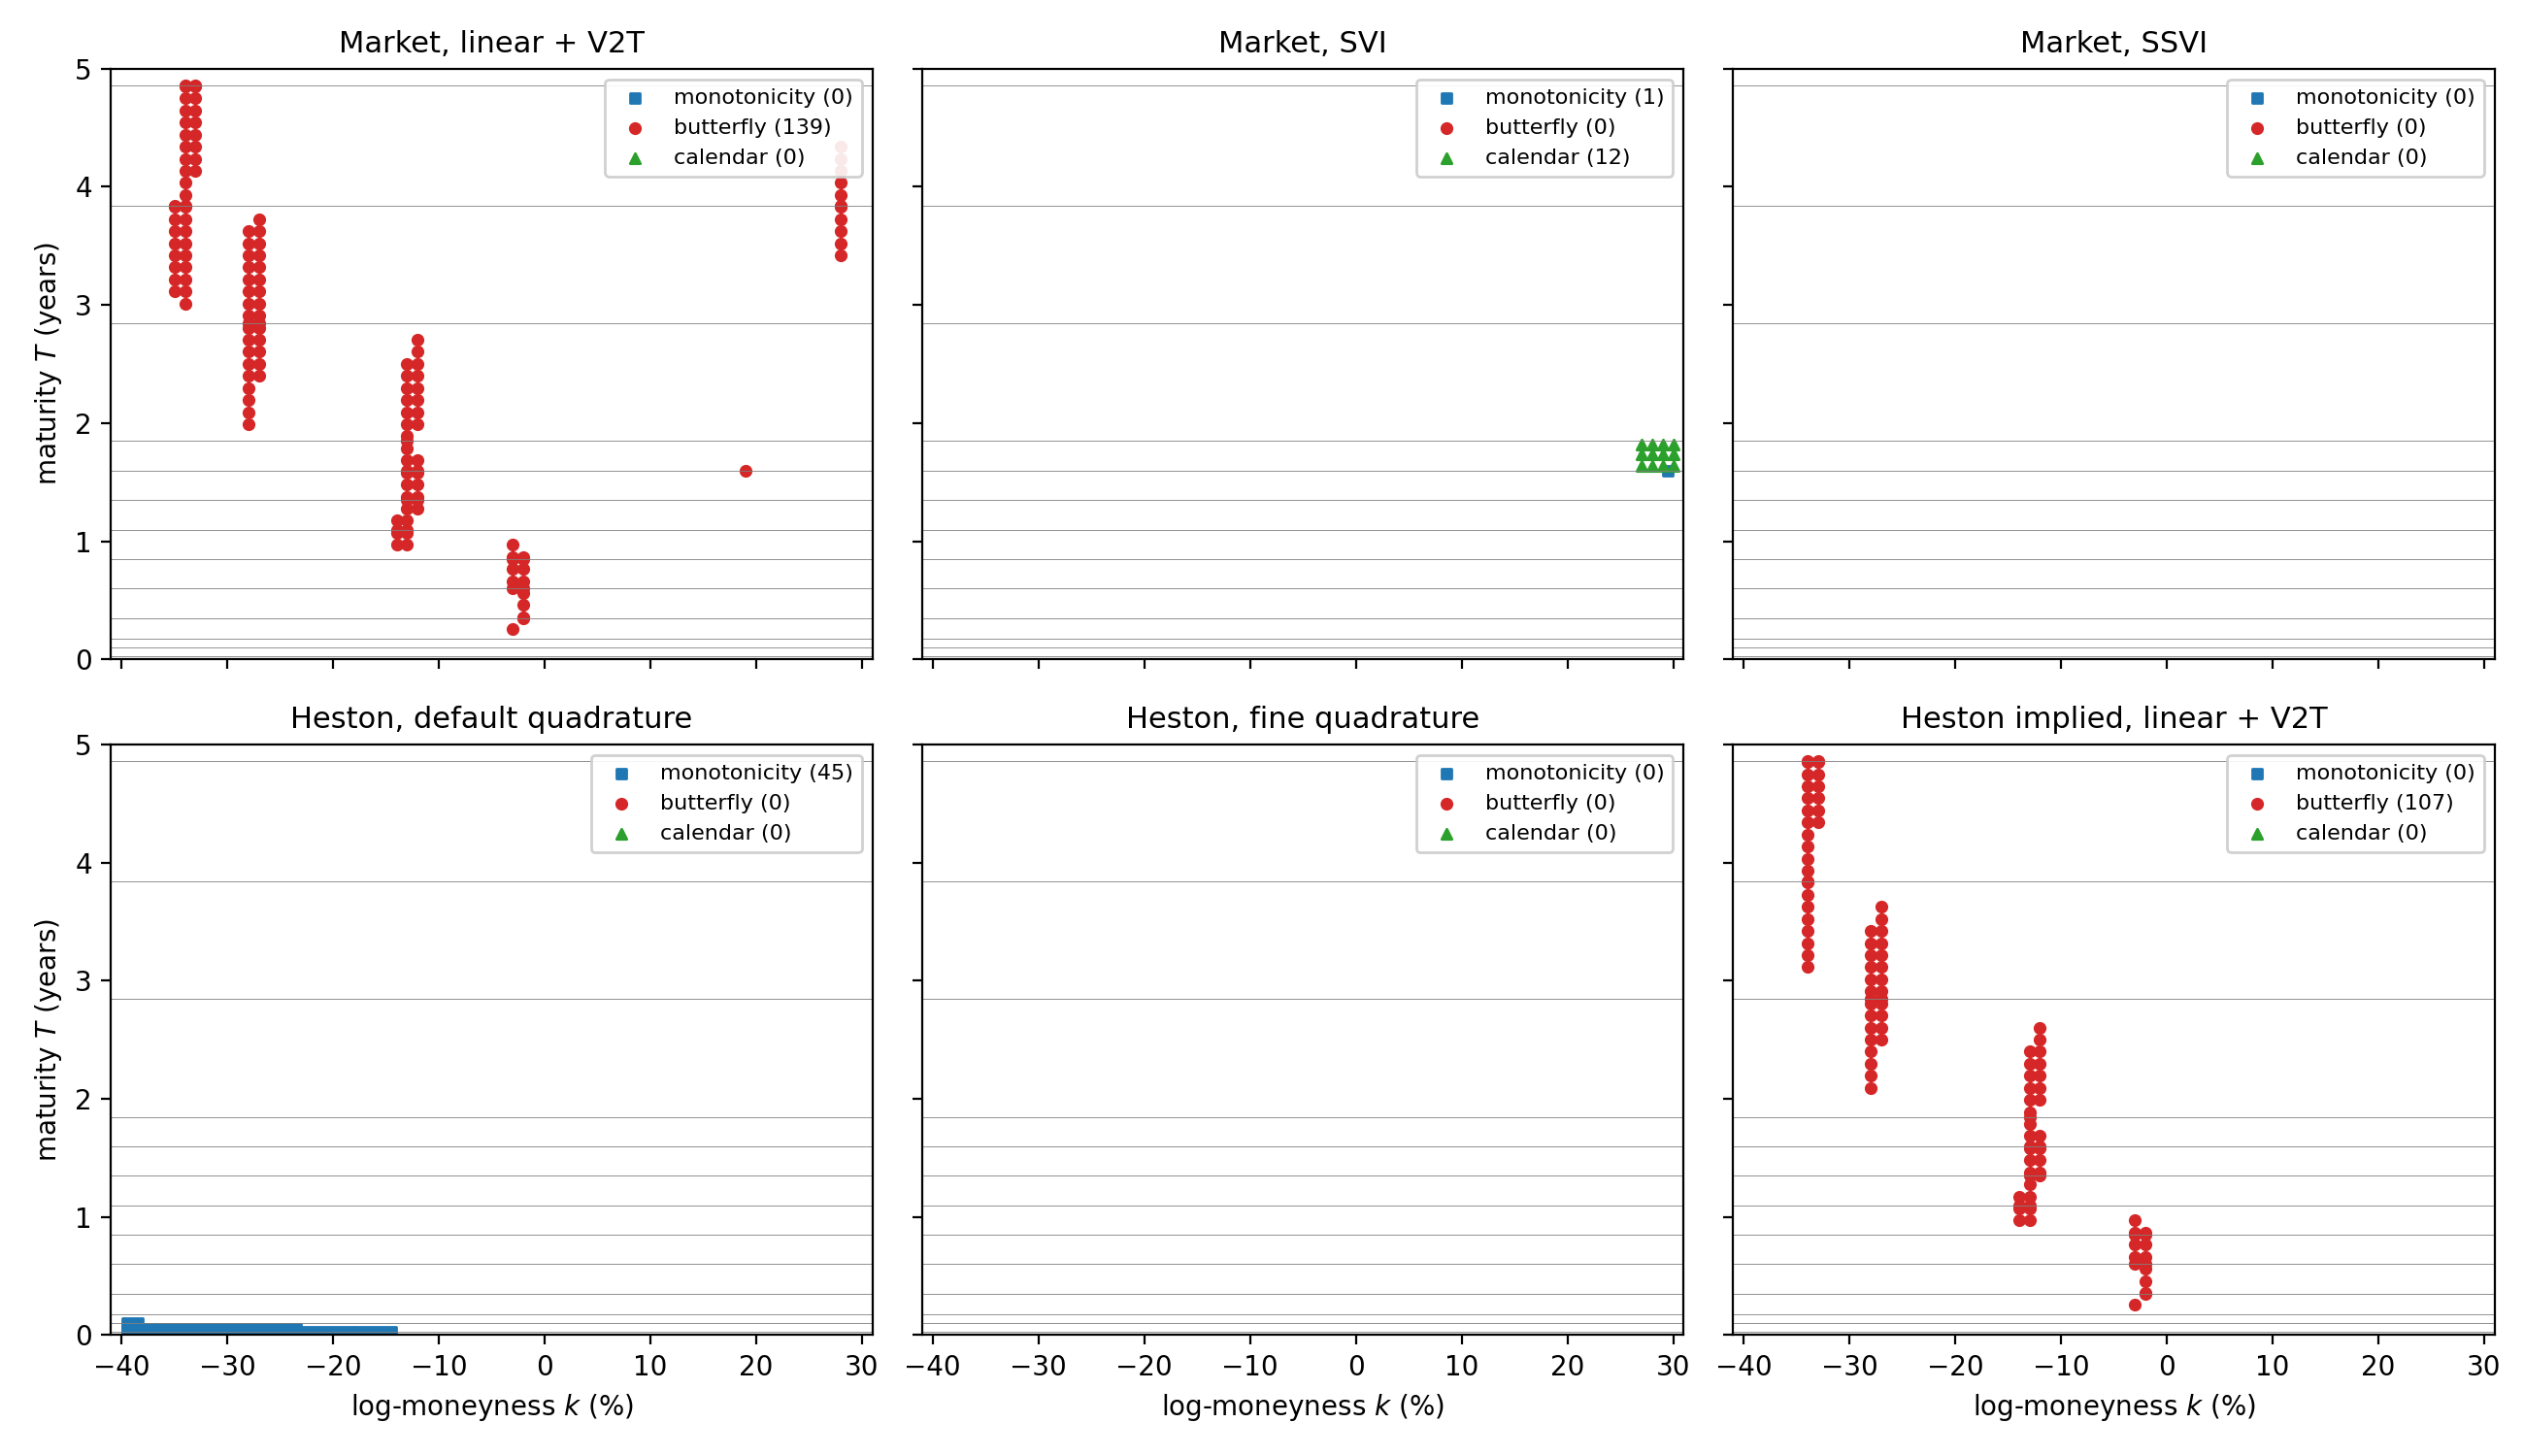
\includegraphics[width=\textwidth]{figures/no_arbitrage_map.png}
\caption{Location of the violations in the $(k, T)$ plane (horizontal lines: listed expiries).}
\label{fig:no_arbitrage_map}
\end{figure}

\subsubsection{Monotonicity}
The interpolated market surfaces satisfy the monotonicity condition everywhere except at one point of the SVI surface,
at $T = 1.60$ and $k = 29.5\%$, where the crossing of two SVI slices described in Section~\ref{sec:calendar_check} also
produces a call price slightly increasing in strike. The Heston model is free of arbitrage by construction, yet the
default quadrature gives 45 violations, all at $T \le 0.1$ year and $k \le -14\%$. There, the out-of-the-money prices are
almost zero and the truncation of the Lewis integral leaves an error of about $-6 \times 10^{-6}$ of the forward (0.05
index point, the order of magnitude found in Section~5.3): Figure~\ref{fig:monotonicity} shows that the default quadrature
even gives slightly negative put prices, while the fine quadrature does not. With the fine quadrature, no violation is
left.

\begin{figure}[h]
\centering
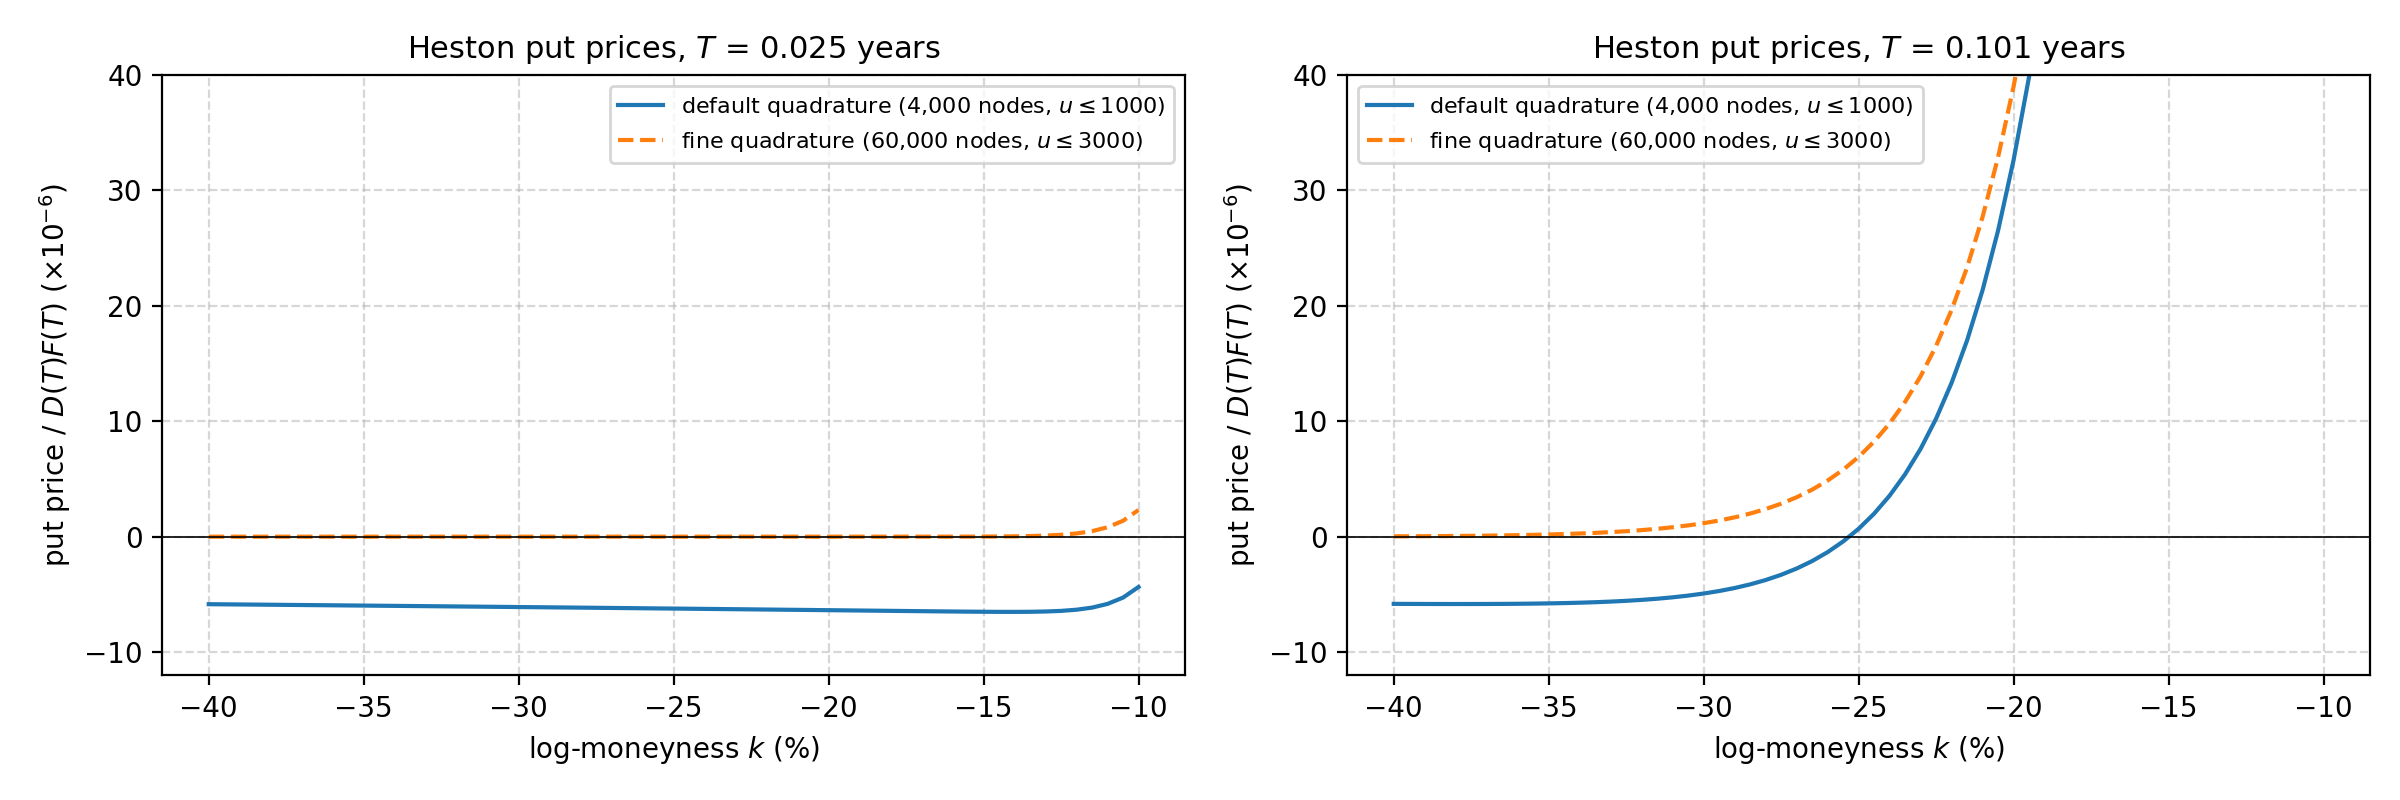
\includegraphics[width=\textwidth]{figures/monotonicity_quadrature.png}
\caption{Heston put prices (normalised) of the far left wing at 9 days and 1 month: the default Lewis quadrature leaves an
error of about $-6 \times 10^{-6}$ of the forward, the fine quadrature none.}
\label{fig:monotonicity}
\end{figure}

\subsubsection{Butterfly}
By the Breeden--Litzenberger identity, the butterfly condition is the positivity of the risk-neutral density
$\partial_{\kappa\kappa}\hat c$ (Figure~\ref{fig:butterfly}). SVI, SSVI and the Heston prices satisfy it everywhere. The linear
interpolation in strike violates it at 139 points (107 on the Heston implied surface), along vertical lines at
$k \approx -35\%, -27\%, -13\%$ and $-3\%$ (Figure~\ref{fig:no_arbitrage_map}). Each line is the lowest quoted strike of a
group of expiries (7800 from 3 to 10 months, 7000 from 1 to 1.8 years, 6000 and 5600 beyond): there, the interpolation
switches from a linear volatility with a negative slope to a flat extrapolation, and the kink makes the density
negative, down to $-15$ at 3.8 years. The linear interpolation also has a kink at every quoted strike, visible as spikes
of the density. Since the Heston implied surface comes from an arbitrage-free model, its 107 violations show that they
are created by the interpolation and not by the data.

\begin{figure}[h]
\centering
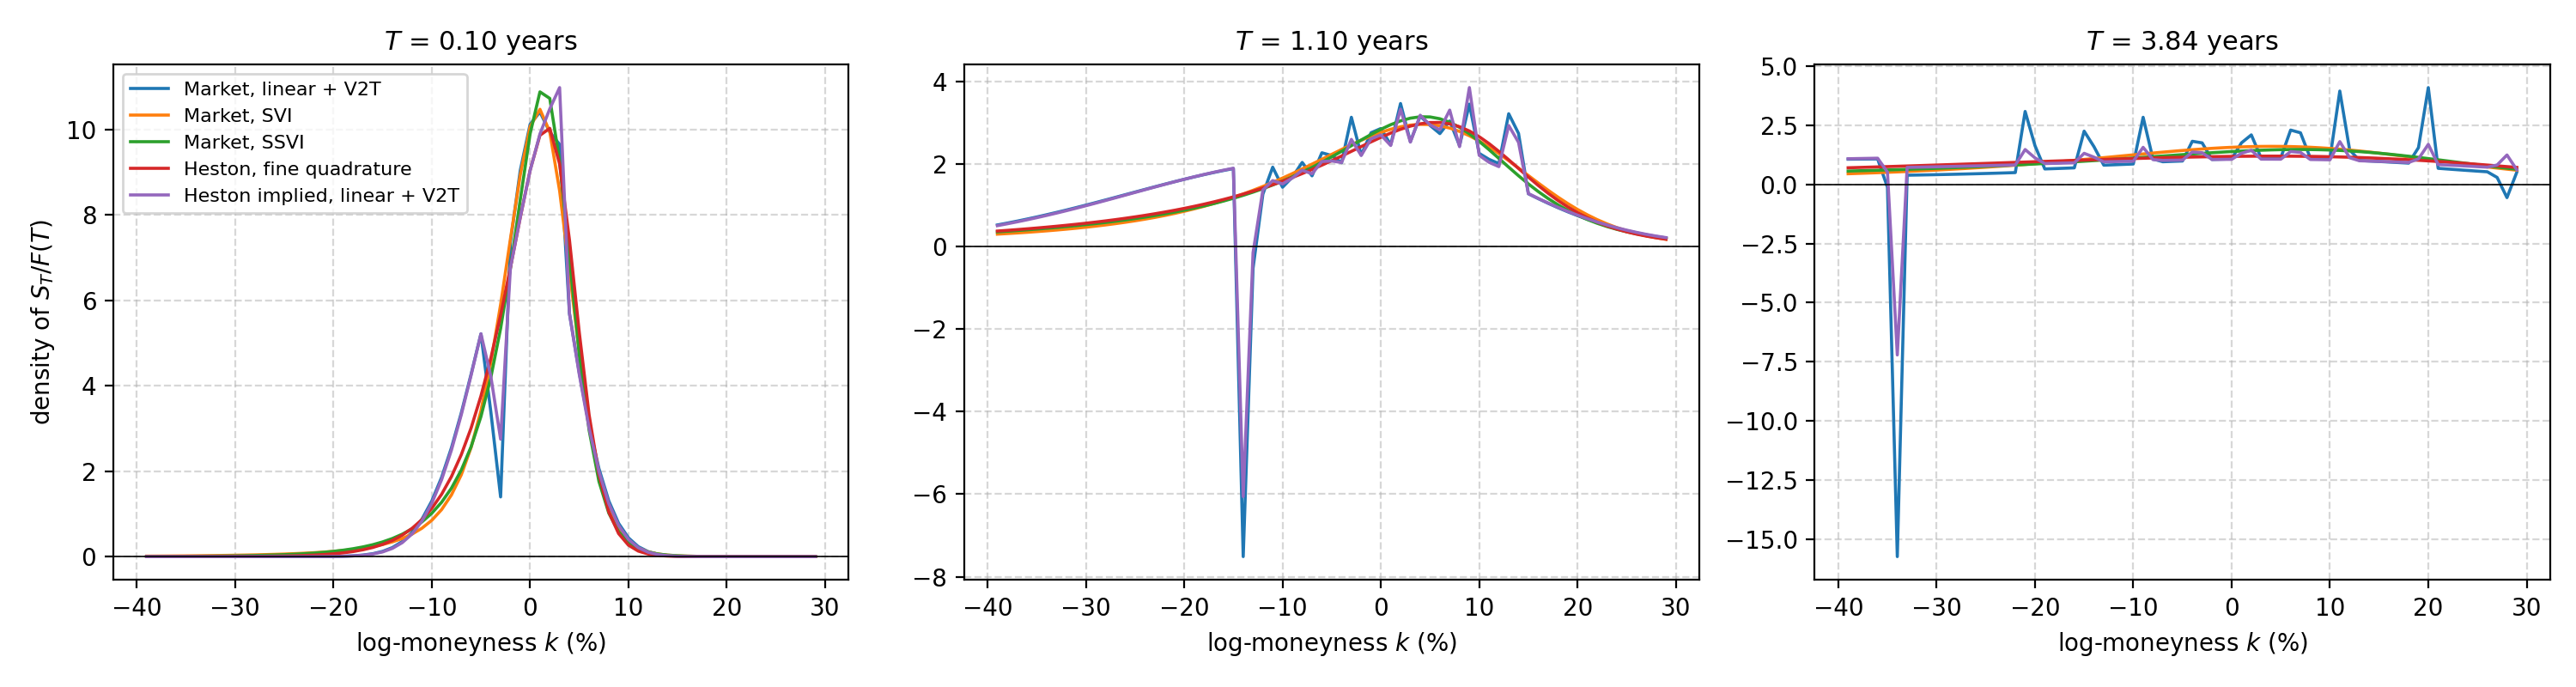
\includegraphics[width=\textwidth]{figures/butterfly_densities.png}
\caption{Risk-neutral densities of $S_T/F(T)$ at 1 month, 1.1 years and 3.8 years.}
\label{fig:butterfly}
\end{figure}

\subsubsection{Calendar}\label{sec:calendar_check}
The linear interpolation in total variance across expiries keeps the calendar condition between the listed expiries,
and SSVI satisfies it by construction ($\theta_T$ non-decreasing). The SVI slices are calibrated independently: the
slices of 1.60 and 1.85 years cross in the right wing (the 1.60-year slice has a positive skew parameter
$\rho = 0.78$, Section~7.5.3), so that the normalised call price decreases between the two expiries for $k \ge 27\%$
(12 violations, Figure~\ref{fig:calendar}). Fitting the slices independently does not guarantee the calendar condition;
SSVI, or SVI slices fitted under calendar constraints, does.

\begin{figure}[h]
\centering
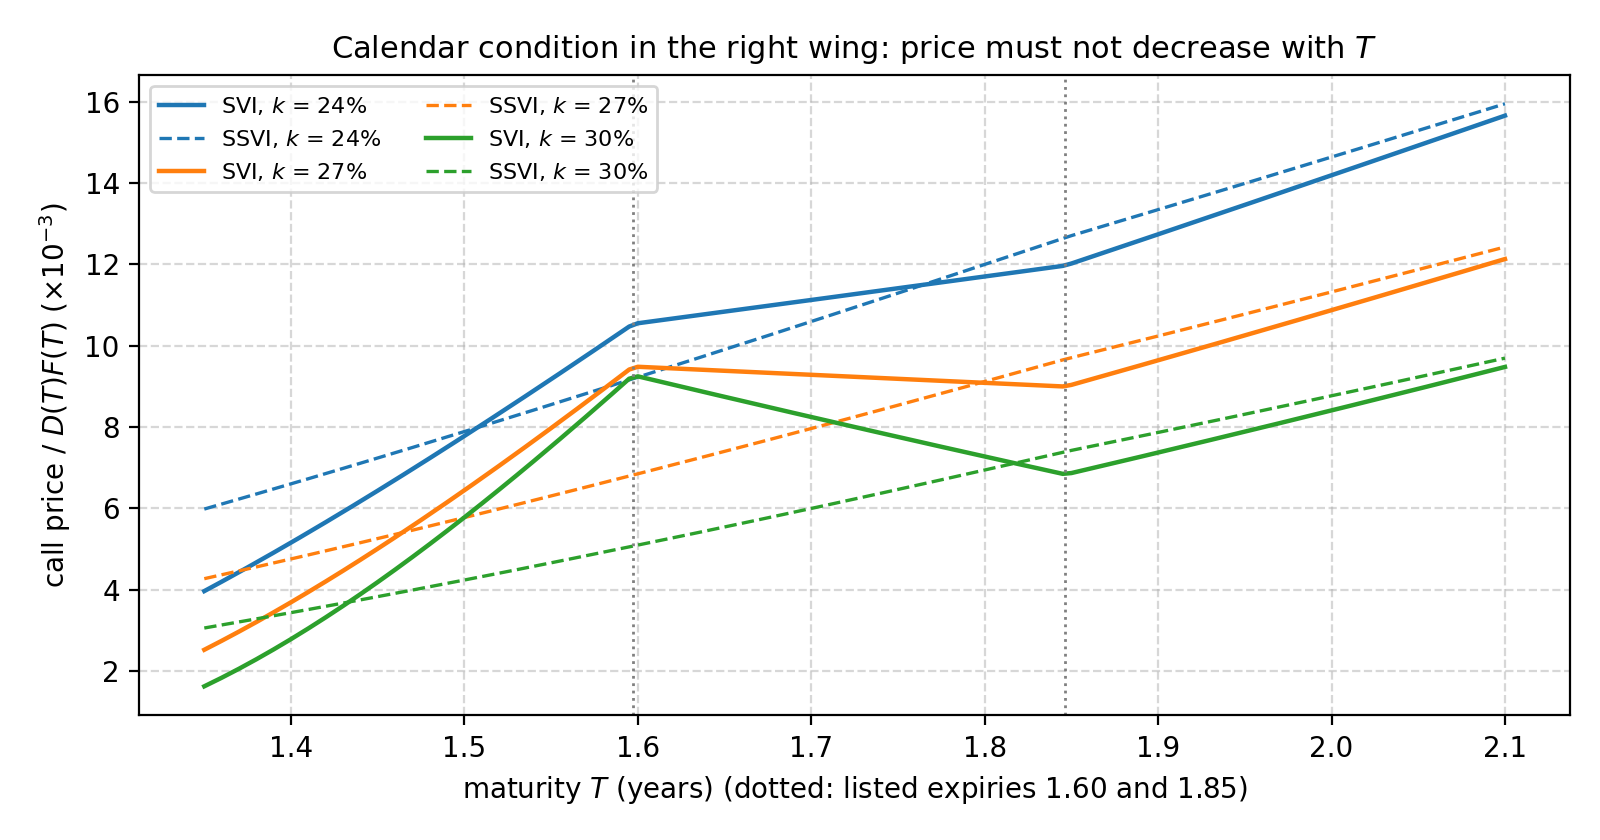
\includegraphics[width=0.8\textwidth]{figures/calendar_svi.png}
\caption{Normalised call prices of the right wing as functions of the maturity: the SVI price decreases between the
1.60 and 1.85-year expiries for $k \ge 27\%$, the SSVI price does not.}
\label{fig:calendar}
\end{figure}

\paragraph{Conclusion.} SSVI is the only interpolation of the market quotes free of static arbitrage on the whole grid.
The linear interpolation in strike, used for the plots of this paper, is adequate for display but creates butterfly
arbitrage at the edges of the quoted strikes: it must not be used to price with a local volatility model, which needs
the second derivative in strike.







\subsection{Monte Carlo sanity check}
As an independent check of the pricer, the semi-analytical price of an ATM call is compared with a Monte Carlo price obtained from \texttt{HestonModel.generate\_paths} (Euler scheme with full truncation, at the calibrated parameters. We take the March 2026 expiry ($T=1.0986$) and $K=8000$, with $250$ time steps and $100{,}000$ paths (seed 42):
\begin{center}
\begin{tabular}{@{}lr@{}}
\toprule
Semi-analytical price (Lewis) & 527.47 \\
Monte Carlo price & $529.35\pm4.41$ (95\%) \\
$\E[S_T]$ (Monte Carlo) & 8039.06 \\
Forward $F(0,T)$ & 8039.09 \\
\bottomrule
\end{tabular}
\end{center}
The difference of $1.88$ is inside the $95\%$ confidence interval, and the simulated mean of $S_T$ matches the forward to $0.03$ points: the drift of the simulation, taken from the forward curve, is consistent with the pricer. The Feller condition is violated at these parameters, so the Euler scheme is biased; the bias is not visible at this level of Monte Carlo noise, but the QE scheme would be preferable for path-dependent products.

\subsection{Diagnostic table}
The empirical exercise suggests the following checklist, linking observable calibration symptoms to their possible upstream causes, in the order in which they should be investigated.

\begin{table}[h]
\centering
\small
\begin{tabular}{@{}p{4.2cm}p{4.6cm}p{5.6cm}@{}}
\toprule
Symptom & Likely upstream cause & Check \\
\midrule
Calls overpriced and puts underpriced at long maturities, growing with $T$ & Overstated forward (missing or too small $q$) & Compare the parity forward $\hat F(T)$ of~\eqref{eq:atmforward} with the forward used in the model \\
$\rho$ close to $-1$, Feller ratio $\ll1$, degenerate $(\kappa,\theta)$ & Forward level error compensated by skew and term structure & Fix the forward first, then recalibrate \\
\texttt{NaN} in the objective, line-search failures & Non-finite model prices or failed implied volatility inversions & Return a finite failure penalty; check the arbitrage bounds of the quotes \\
Very different parameters for almost the same loss, erratic parameters across days & Flat valley, ill-posed inverse problem & Multi-start; compute $\operatorname{cond}(J^\top J)$; Tikhonov regularization toward the previous day \\
Bad fit only below one month & Structural limit of a diffusion with constant parameters & Time-dependent $\xi$ and $\rho$ (Section~\ref{sec:td}) or a jump extension (Bates) \\
\bottomrule
\end{tabular}
\caption{Diagnostic table for Heston calibration on equity index options.}
\label{tab:diag}
\end{table}



\clearpage
% ===============================================================
\section{Time-Dependent Heston Model}
\label{sec:td}
% ===============================================================

As we have seen in Section~\ref{sec:results}, the RMSE of the constant Heston model is concentrated at both ends of the surface: $0.53$ vol points at 9 days and $0.64$--$0.81$ beyond 2.8 years (Table~\ref{tab:errors}). The optimization is not the cause, since the global searches of Section~\ref{sec:global} all reach the same minimum. With five constant parameters, the model cannot fit the whole surface: the ATM skew is bounded at short maturities by $\rho\xi/(4\sqrt{v_0})$~\eqref{eq:smallskew}, and a single pair $(\kappa,\theta)$ must describe the whole term structure of variance. Without changing the data, we therefore enrich the model: instead of taking the parameters constant, we make them piecewise constant in time.

\subsection{Dynamics}
Following Mikhailov and N\"ogel~\cite{mikhailov} (see also Benhamou, Gobet and Miri~\cite{hestontd}), the variance follows
\begin{equation}
    \dd v_t = \kappa\,\bigl(\theta(t) - v_t\bigr)\,\dd t + \xi(t)\sqrt{v_t}\,\dd W^v_t, \qquad \dd\langle W^S, W^v\rangle_t = \rho(t)\,\dd t,
    \label{eq:td-sde}
\end{equation}
with $\theta$, $\xi$ and $\rho$ constant on each interval $(T_{j-1},T_j]$ between two listed expiries ($T_0=0$, $j=1,\dots,13$), and keeping their last value beyond $T_{13}$; $v_0$ and $\kappa$ are global. The spot dynamics~\eqref{eq:sde-S} are unchanged. With identical values on every interval, the model is the constant Heston model.

We compare two families:
\begin{itemize}
    \item $\theta(t)$ only: $v_0$, $\kappa$ and 13 values of $\theta$, with $\xi$ and $\rho$ kept at their constant calibration, i.e. 15 parameters;
    \item $(\theta,\xi,\rho)(t)$: $v_0$, $\kappa$ and 13 values of each of $\theta$, $\xi$, $\rho$, i.e. 41 parameters, for 142 quotes.
\end{itemize}

\subsection{Characteristic function}
The model remains affine. The characteristic function of $X_T=\ln(S_T/F(T))$ is still $\phi_X(u;T)=\exp\bigl(C(u,T)+D(u,T)\,v_0\bigr)$, but the Riccati system~\eqref{eq:D}--\eqref{eq:C} now has piecewise constant coefficients. It is solved backward in time, from $T$ to $0$, interval by interval. On an interval of length $\tau$ with parameters $(\theta,\xi,\rho)$ and terminal values $(C_0,D_0)$ (with $C_0=D_0=0$ on the last interval before $T$), let $\beta=\kappa-\iu\rho\xi u$, $d=\sqrt{\beta^2+\xi^2(u^2+\iu u)}$ and
\begin{equation}
    g=\frac{\beta-d-\xi^2D_0}{\beta+d-\xi^2D_0}.
\end{equation}
Then
\begin{align}
    D &= D_0+\frac{\beta-d-\xi^2D_0}{\xi^2}\,\frac{1-e^{-d\tau}}{1-g\,e^{-d\tau}}, \label{eq:td-D}\\
    C &= C_0+\frac{\kappa\theta}{\xi^2}\left[(\beta-d)\,\tau-2\ln\frac{1-g\,e^{-d\tau}}{1-g}\right]. \label{eq:td-C}
\end{align}
For $D_0=0$ these are exactly~\eqref{eq:D}--\eqref{eq:C}. The Lewis formula~\eqref{eq:lewis} is unchanged, and a price at $T_j$ costs $j$ evaluations of~\eqref{eq:td-D}--\eqref{eq:td-C} instead of one: a loss evaluation on the 13 expiries takes about $55$ ms against $26$ ms for the constant model. With the same parameters on every interval, the implementation (\texttt{TimeDependentHestonModel} in \texttt{Heston.py}, a subclass of \texttt{HestonModel}) reproduces the constant characteristic function to $3\times10^{-16}$.

\subsection{Calibration}
The calibration process is organized into three steps, all on the loss~\eqref{eq:loss-iv} and with the same bounds~\eqref{eq:bounds}; $\kappa$ and $v_0$ start from the constant calibration of Section~\ref{sec:global}.
\begin{enumerate}
    \item \textbf{Bootstrap.} For $j=1,\dots,13$, the parameters of interval $j$ are fitted by L-BFGS-B to the smile of $T_j$ alone, the earlier intervals being fixed; $v_0$ is fitted with the first expiry and $\kappa$ is kept. Each step has one ($\theta$) or three ($\theta,\xi,\rho$) parameters for 11 quotes. The whole bootstrap takes $0.6$ s ($\theta$) or $3.2$ s ($\theta,\xi,\rho$). It is greedy: each interval absorbs the errors left by the previous ones.
    \item \textbf{Global calibration.} All the parameters ($v_0$, $\kappa$ and the time-dependent ones) are fitted jointly on the 13 expiries, starting from the bootstrap. With finite-difference gradients, this takes $84$ s for 15 parameters and $143$ s for 41.
    \item \textbf{Global calibration with smoothness.} To avoid parameters that jump from one interval to the next, we add the penalty
    \begin{equation}
        \lambda\sum_{p\in\{\theta,\xi,\rho\}}\sum_{j=2}^{13}\left(\frac{p_j-p_{j-1}}{b_p-a_p}\right)^2,\qquad\lambda=10^{-4},
        \label{eq:smoothness}
    \end{equation}
    with $[a_p,b_p]$ the bounds of $p$, and restart from the unpenalized optimum. The run stops at the limit of 150 iterations after $423$ s.
\end{enumerate}

\subsection{Results}
Table~\ref{tab:td_errors} gives the implied volatility RMSE per expiry, after exact inversion of the model prices.

\begin{table}[htbp]
\centering
\small
\begin{tabular}{@{}rrrrrrr@{}}
\toprule
 & Heston & \multicolumn{2}{c}{$\theta(t)$} & \multicolumn{3}{c}{$(\theta,\xi,\rho)(t)$} \\
\cmidrule(lr){3-4}\cmidrule(l){5-7}
$T$ & constant & bootstrap & global & bootstrap & global & global + smooth. \\
\midrule
0.025 & 0.527 & 0.199 & 0.196 & 0.037 & 0.038 & 0.163 \\
0.101 & 0.126 & 0.122 & 0.137 & 0.047 & 0.065 & 0.139 \\
0.178 & 0.124 & 0.114 & 0.137 & 0.101 & 0.122 & 0.074 \\
0.351 & 0.240 & 0.065 & 0.105 & 0.055 & 0.082 & 0.065 \\
0.600 & 0.268 & 0.045 & 0.095 & 0.017 & 0.078 & 0.081 \\
0.849 & 0.276 & 0.016 & 0.097 & 0.017 & 0.062 & 0.049 \\
1.099 & 0.109 & 0.067 & 0.222 & 0.106 & 0.117 & 0.181 \\
1.348 & 0.208 & 0.106 & 0.182 & 0.109 & 0.119 & 0.156 \\
1.597 & 0.192 & 0.156 & 0.218 & 0.208 & 0.124 & 0.204 \\
1.847 & 0.222 & 0.126 & 0.278 & 0.151 & 0.108 & 0.238 \\
2.844 & 0.640 & 0.605 & 0.452 & 0.324 & 0.178 & 0.182 \\
3.841 & 0.793 & 0.774 & 0.551 & 0.339 & 0.222 & 0.138 \\
4.858 & 0.811 & 0.637 & 0.306 & 0.132 & 0.075 & 0.110 \\
\midrule
RMSE & 0.421 & 0.337 & 0.265 & 0.163 & 0.118 & 0.148 \\
Max & 1.749 & 1.824 & 1.080 & 0.794 & 0.520 & 0.527 \\
Parameters & 5 & 14 & 15 & 40 & 41 & 41 \\
\bottomrule
\end{tabular}
\caption{Implied volatility RMSE per expiry (vol points, exact inversion) of the constant and time-dependent Heston models. The bootstraps keep $\kappa$ fixed, hence one parameter less.}
\label{tab:td_errors}
\end{table}

\begin{itemize}
    \item \emph{$\theta(t)$ only.} The global calibration lowers the RMSE from $0.421$ to $0.265$ vol points and the maximum error from $1.75$ to $1.08$. The gain comes from the long maturities ($0.64$--$0.81$ down to $0.31$--$0.55$): $\theta(t)$ fixes the term structure of the ATM level. It does not fix the short-maturity skew, which depends on $\xi$ and $\rho$: $0.20$ vol points are left at 9 days.
    \item \emph{$(\theta,\xi,\rho)(t)$.} The RMSE falls to $0.163$ (bootstrap), $0.118$ (global) and $0.148$ (global with smoothness), i.e. $2.6$ to $3.6$ times less than the constant model, with a maximum error of $0.52$ vol points. Without penalty, the 9-day smile is fitted to $0.04$ vol points, against $0.53$ for the constant model: a short first interval with its own $\xi$ and $\rho$ removes the bound~\eqref{eq:smallskew} on the short-maturity skew.
\end{itemize}

Figure~\ref{fig:td_params} shows the calibrated parameters. Without penalty, they jump from one interval to the next; the bootstrap even gives $\rho=-0.995$ on $(0.178,0.351]$ and $\xi$ at its upper bound $5$ beyond 1.85 years. The fit is partly obtained by over-parametrization (Section~\ref{sec:td_validation}). With the smoothness penalty~\eqref{eq:smoothness}, the term structures are regular (Table~\ref{tab:td_smooth}) for $0.03$ vol points of RMSE: $\rho(t)$ stays between $-0.70$ and $-0.46$; $\theta(t)$ decreases from $0.13$ to $0.03$ on $(0.6,0.85]$ then rises to $0.16$; $\xi(t)$ falls to $0.25$ around $0.7$ years, then rises to $3.3$ at 5 years. Figure~\ref{fig:td_smiles} compares the smiles.

\begin{figure}[htbp]
    \centering
    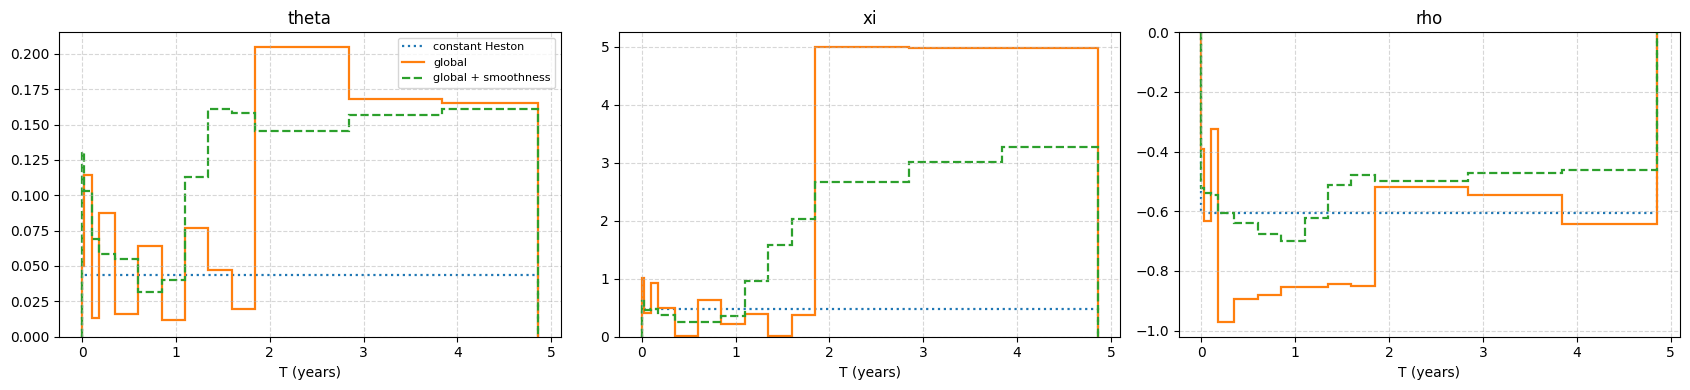
\includegraphics[width=\textwidth]{figures/td_parameters.png}
    \caption{Piecewise constant parameters $\theta(t)$, $\xi(t)$, $\rho(t)$: constant Heston (dotted), global calibration without penalty (solid) and with smoothness (dashed).}
    \label{fig:td_params}
\end{figure}

\begin{table}[htbp]
\centering
\small
\begin{tabular}{@{}rrrrrr@{}}
\toprule
Interval & $\theta$ & $\xi$ & $\rho$ & $\sqrt{\theta}$ & $2\kappa\theta/\xi^2$ \\
\midrule
$(0, 0.025]$     & 0.1304 & 0.6185 & $-0.5206$ & 36.1\% & 0.443 \\
$(0.025, 0.101]$ & 0.1032 & 0.4644 & $-0.5395$ & 32.1\% & 0.621 \\
$(0.101, 0.178]$ & 0.0693 & 0.4707 & $-0.5454$ & 26.3\% & 0.406 \\
$(0.178, 0.351]$ & 0.0587 & 0.3668 & $-0.6051$ & 24.2\% & 0.567 \\
$(0.351, 0.600]$ & 0.0548 & 0.2615 & $-0.6384$ & 23.4\% & 1.040 \\
$(0.600, 0.849]$ & 0.0318 & 0.2453 & $-0.6763$ & 17.8\% & 0.687 \\
$(0.849, 1.099]$ & 0.0403 & 0.3594 & $-0.6982$ & 20.1\% & 0.405 \\
$(1.099, 1.348]$ & 0.1129 & 0.9615 & $-0.6240$ & 33.6\% & 0.159 \\
$(1.348, 1.597]$ & 0.1608 & 1.5786 & $-0.5111$ & 40.1\% & 0.084 \\
$(1.597, 1.847]$ & 0.1580 & 2.0344 & $-0.4799$ & 39.7\% & 0.050 \\
$(1.847, 2.844]$ & 0.1453 & 2.6591 & $-0.4977$ & 38.1\% & 0.027 \\
$(2.844, 3.841]$ & 0.1565 & 3.0181 & $-0.4720$ & 39.6\% & 0.022 \\
$(3.841, 4.858]$ & 0.1609 & 3.2667 & $-0.4620$ & 40.1\% & 0.020 \\
\bottomrule
\end{tabular}
\caption{Time-dependent parameters calibrated with smoothness ($v_0=0.0183$, $\kappa=0.649$).}
\label{tab:td_smooth}
\end{table}

\begin{figure}[htbp]
    \centering
    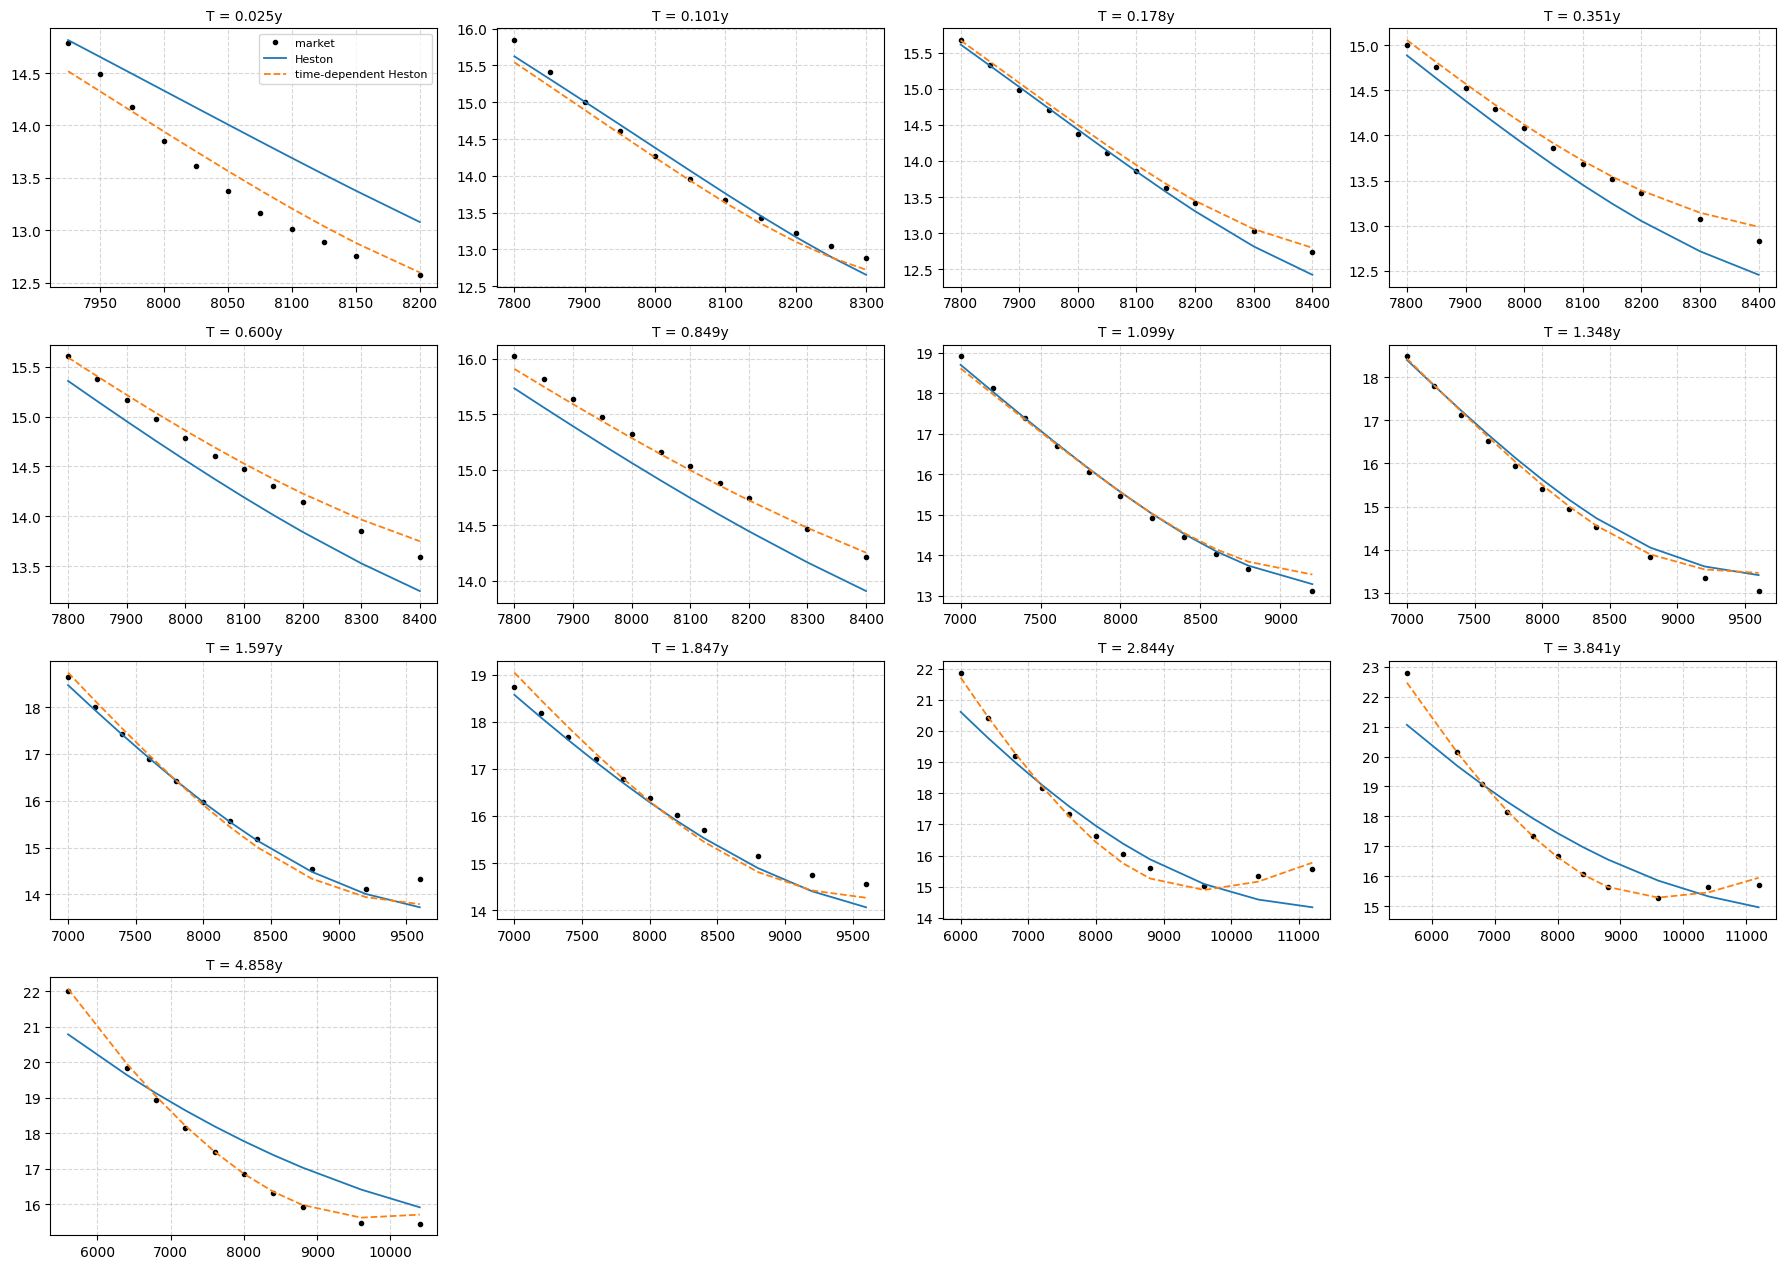
\includegraphics[width=\textwidth]{figures/td_smiles.png}
    \caption{Market implied volatilities (dots), constant Heston (solid) and time-dependent Heston with smoothness (dashed) at the quoted strikes.}
    \label{fig:td_smiles}
\end{figure}

The price of the fit is the vol-of-vol: beyond 1.6 years, $\xi(t)$ reaches $2$--$3.3$ and the Feller ratio falls to $0.02$--$0.05$. The variance then spends more time near zero, which matters for path-dependent products, and the full-truncation Euler scheme becomes biased. Table~\ref{tab:td_mc} compares the Lewis prices of the smooth model with Monte Carlo prices (400 steps, 200{,}000 antithetic paths) at $T=1.5973$: the puts agree, but the calls exceed the Lewis prices by $2.3$ to $2.6$ standard errors. The gap of the ATM call decreases with the number of steps ($+15.1$ with 100 steps, $+4.6$ with 400, $+3.1$ with 1{,}600), so it comes from the discretization and not from the pricer; the QE scheme~\cite{andersen} would be needed for path-dependent products.

\begin{table}[htbp]
\centering
\small
\begin{tabular}{@{}rlrrr@{}}
\toprule
Strike & Type & Lewis & Monte Carlo & Std. error \\
\midrule
6500 & put  & 219.50 & 219.93 & 1.48 \\
7500 & put  & 454.89 & 456.00 & 2.13 \\
8000 & call & 589.20 & 593.70 & 1.93 \\
8500 & call & 361.48 & 365.69 & 1.60 \\
9500 & call & 115.96 & 118.23 & 1.01 \\
\bottomrule
\end{tabular}
\caption{Time-dependent model with smoothness: Lewis prices against Euler full-truncation Monte Carlo ($T=1.5973$, 400 steps, 200{,}000 antithetic paths).}
\label{tab:td_mc}
\end{table}

\subsection{Out-of-sample and stability tests}
\label{sec:td_validation}
A lower in-sample error with 41 parameters for 142 quotes does not prove a better model. Two tests tell a better model from an overfitted one:
\begin{enumerate}
    \item \textbf{Out-of-sample errors.} The models are calibrated without some quotes, and the error is measured on them. An overfitted model has a small in-sample error and a large out-of-sample one. We use two splits:
    \begin{itemize}
        \item \emph{leave-one-expiry-out}: each of the 13 expiries is left out in turn. The intervals of the time-dependent models then end at the 12 remaining expiries, and the left-out expiry is priced with the parameters of the merged interval: this tests the interpolation in time (extrapolation for the last expiry);
        \item \emph{strike holdout}: one strike out of two is left out at every expiry, and the two complementary splits are pooled (77 and 65 calibration quotes). This tests the interpolation in strike.
    \end{itemize}
    \item \textbf{Stability under noise.} The market implied volatilities are perturbed by an i.i.d.\ Gaussian noise of standard deviation $\sigma=0.1$ vol points, of the order of a bid-ask half-spread, and the models are recalibrated (20 draws). For a linear least-squares fit with $k$ parameters and $n=142$ quotes, the noise moves the fitted values by $\sigma\sqrt{k/n}$ on average. A model that fits the noise moves its surface and its parameters much more.
\end{enumerate}
Every test reruns the whole procedure (bootstrap, global calibration, smoothness) on the modified data, starting from the constant model, so that no information from the left-out quotes leaks into the starting point. The only exception is the constant model, run locally from the global minimum of Section~\ref{sec:global}, which is unique. The 35 calibrations (5 models each) are independent and run in parallel (\texttt{calibration\_validation.py}, joblib): 53 minutes on 20 cores.

\begin{table}[htbp]
\centering
\small
\resizebox{\textwidth}{!}{%
\begin{tabular}{@{}lrrrrrrrr@{}}
\toprule
 & & & \multicolumn{2}{c}{Out of sample} & \multicolumn{4}{c}{Noise $\sigma=0.1$ (20 draws)} \\
\cmidrule(lr){4-5}\cmidrule(l){6-9}
Model & $k$ & In-sample & Expiry left out & Strikes left out & Fit to noisy quotes & Error vs original & Displacement & $\sigma\sqrt{k/n}$ \\
\midrule
Heston constant              & 5  & 0.421 & 0.516 & 0.462 & 0.433 & 0.422 & 0.017 & 0.019 \\
$\theta(t)$, global          & 15 & 0.265 & 0.343 & 0.338 & 0.282 & 0.269 & 0.040 & 0.033 \\
$(\theta,\xi,\rho)(t)$, bootstrap & 40 & 0.163 & 0.387 & 0.185 & 0.261 & 0.247 & 0.270 & 0.053 \\
$(\theta,\xi,\rho)(t)$, global    & 41 & 0.118 & 0.352 & 0.148 & 0.166 & 0.147 & 0.141 & 0.054 \\
$(\theta,\xi,\rho)(t)$, global + smoothness & 41 & 0.148 & \textbf{0.245} & \textbf{0.136} & 0.191 & 0.170 & 0.145 & 0.054 \\
\bottomrule
\end{tabular}}
\caption{Out-of-sample and stability tests (implied volatility RMSE in vol points). Displacement: RMSE between the implied volatilities of the model calibrated on noisy quotes and on the original quotes.}
\label{tab:td_validation}
\end{table}

\paragraph{Strikes: no overfitting.} On the strike holdout, the error on the left-out strikes is $0.9$ to $1.3$ times the error on the calibration strikes for every model ($1.14$ for the constant model, $1.10$ with smoothness). The full models keep their advantage out of sample ($0.136$--$0.185$ vol points against $0.462$): three parameters per smile of 11 quotes do not fit the noise in the strike direction.

\paragraph{Maturities: real degradation.} Leaving one expiry out (Figure~\ref{fig:td_loo}), the constant model goes from $0.42$ to $0.52$ vol points, $\theta(t)$ from $0.27$ to $0.34$, the full global model from $0.12$ to $0.35$, three times its in-sample error, and the full bootstrap from $0.16$ to $0.39$. Out of sample, the 26 additional parameters of the full global model bring nothing over $\theta(t)$ ($0.352$ against $0.343$): the parameters of one interval say little about the next one. With smoothness, the out-of-sample error is the lowest ($0.245$, half the error of the constant model): it is the penalty that makes the time-dependent parameters interpolate. The 9-day expiry is the hardest to predict for the constant and full models ($0.55$ to $0.92$ vol points), since its skew is far from the next one; $\theta(t)$ predicts it to $0.19$, since its $\xi$ and $\rho$ are fitted on the whole surface.

\begin{figure}[htbp]
    \centering
    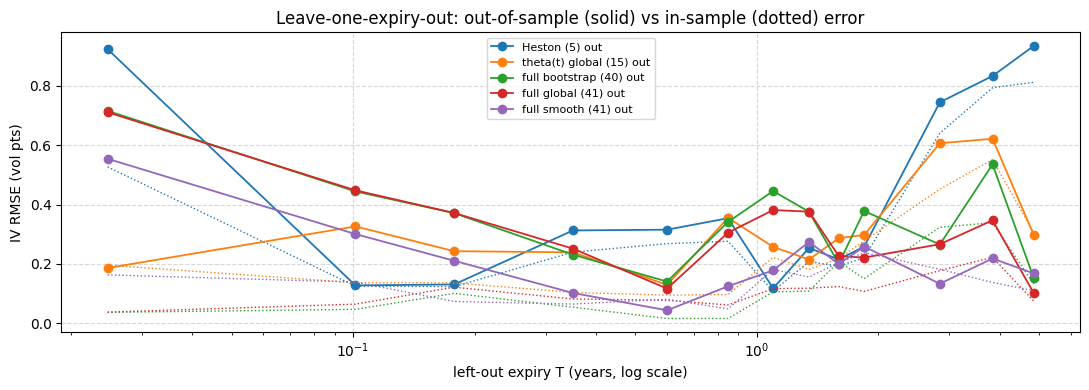
\includegraphics[width=\textwidth]{figures/td_leave_one_expiry_out.png}
    \caption{Leave-one-expiry-out: out-of-sample error at the left-out expiry (solid) against the in-sample error at the same expiry (dotted).}
    \label{fig:td_loo}
\end{figure}

\paragraph{Noise: the full models are unstable.} For the constant model and $\theta(t)$, the noise moves the fitted surface by $0.017$ and $0.040$ vol points, close to the least-squares reference $\sigma\sqrt{k/n}$, and the parameters barely move (standard deviation of $\kappa$: $0.03$--$0.04$). For the full models, the surface moves by $0.14$--$0.27$ vol points, $2.6$ to $5$ times the reference and more than the noise itself, and the parameters jump from one draw to the next (Table~\ref{tab:td_dispersion}, Figure~\ref{fig:td_noise}). Yet their fit to the noisy quotes ($0.17$--$0.26$) is not below the least-squares reference $\sqrt{e^2+\sigma^2(1-k/n)}$, $e$ being the in-sample error ($0.15$--$0.18$ for these models): the models do not absorb the noise, the optimizer lands in different minima of a flat loss. This is a lack of identifiability rather than overfitting in the classical sense, the same phenomenon as the $(\kappa,\xi)$ valley of the constant model (Section~\ref{sec:global}), with many more directions. The smoothness penalty stabilizes $\rho$ (median standard deviation $0.06$ against $0.21$) and halves the dispersion of $\xi$, but not the displacement of the surface. The bootstrap is the least stable: each interval inherits the errors of the previous ones.

\begin{table}[htbp]
\centering
\small
\begin{tabular}{@{}lrrrrrrrr@{}}
\toprule
 & & & \multicolumn{2}{c}{$\theta$} & \multicolumn{2}{c}{$\xi$} & \multicolumn{2}{c}{$\rho$} \\
\cmidrule(lr){4-5}\cmidrule(lr){6-7}\cmidrule(l){8-9}
Model & $v_0$ & $\kappa$ & median & max & median & max & median & max \\
\midrule
Heston constant              & 0.0001 & 0.033 & 0.0003 & 0.0003 & 0.005 & 0.005 & 0.002 & 0.002 \\
$\theta(t)$, global          & 0.0001 & 0.038 & 0.0070 & 0.0103 & 0.005 & 0.005 & 0.002 & 0.002 \\
$(\theta,\xi,\rho)(t)$, bootstrap & 0.0005 & 0.033 & 0.0245 & 0.0549 & 0.631 & 1.885 & 0.234 & 0.362 \\
$(\theta,\xi,\rho)(t)$, global    & 0.0004 & 0.447 & 0.0620 & 0.2415 & 0.657 & 1.823 & 0.209 & 0.357 \\
$(\theta,\xi,\rho)(t)$, smoothness & 0.0005 & 0.545 & 0.0599 & 0.1138 & 0.359 & 0.996 & 0.062 & 0.267 \\
\bottomrule
\end{tabular}
\caption{Standard deviation of the calibrated parameters over the 20 noisy draws. For the time-dependent parameters: median and maximum over the 13 intervals.}
\label{tab:td_dispersion}
\end{table}

\begin{figure}[htbp]
    \centering
    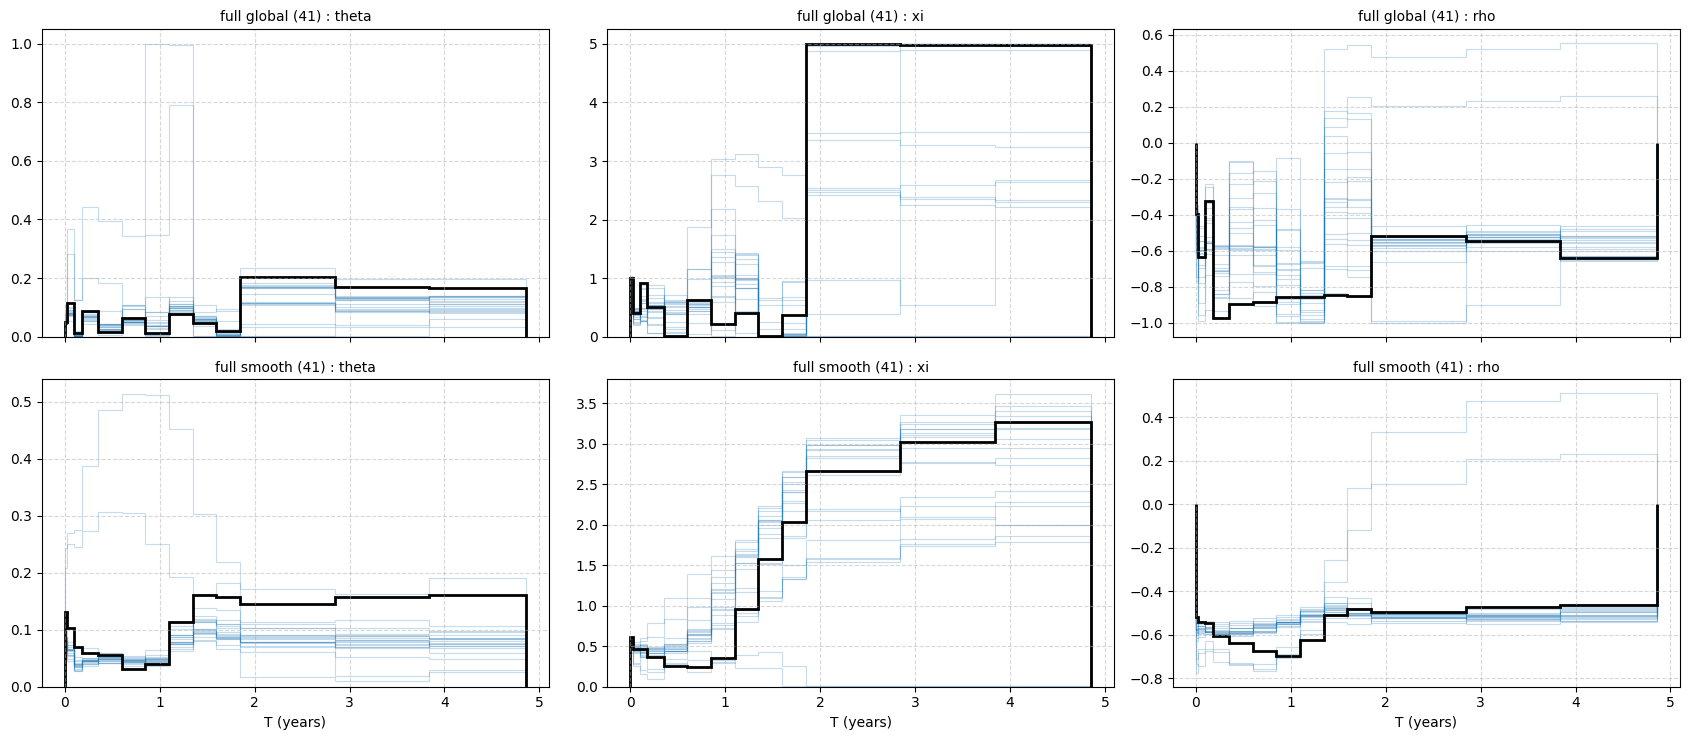
\includegraphics[width=\textwidth]{figures/td_noise_parameters.png}
    \caption{Parameters recalibrated on the 20 noisy draws (thin lines) around the parameters calibrated on the original quotes (thick line), without (top) and with (bottom) smoothness.}
    \label{fig:td_noise}
\end{figure}

\paragraph{Conclusion of the tests.} $\theta(t)$ is a safe improvement: from $0.52$ to $0.34$ vol points out of sample, as stable as the constant model. The full time-dependent model fits better in-sample and between strikes, but its parameters are not identified by the vanilla quotes of a single day. It needs the smoothness penalty to interpolate in time, and even then its parameters and its surface depend on the noise of the quotes. Since exotic products depend on the forward skew and on the vol-of-vol, two calibrations that agree on the vanillas within a few hundredths of a vol point can give different exotic prices.


% ===============================================================
\section{Next Steps}
\label{sec:next-steps}
% ===============================================================

\begin{itemize}
    \item Recalibrate on several consecutive valuation dates, and use the Tikhonov penalty toward the previous day's parameters to measure the gain in parameter stability.
    \item Add analytical gradients (Section~\ref{sec:pricing}) to replace finite differences in L-BFGS-B, and analytical first- and second-order Greeks to the \texttt{HestonModel} class. For the time-dependent model, finite differences over 41 parameters are the bottleneck (7 minutes per calibration).
    \item Implement the Carr--Madan FFT and the COS method, and compare their speed and accuracy with the Lewis quadrature.
    \item Compute the Jacobian $J$ of the residuals at the optimum and the condition number of $J^\top J$ to quantify the flat valley of Section~\ref{sec:global}.
    \item Implement the Quadratic-Exponential scheme (Andersen, 2008) as a more accurate alternative to Euler full truncation when the Feller condition is violated.
    \item Add the parity regression estimator of the forward and a smoothing of the short-maturity carry.
    \item Reduce the number of effective parameters of the time-dependent model: $\xi$ and $\rho$ on three or four coarse maturity buckets instead of 13 intervals, or a stronger smoothness penalty chosen by leave-one-expiry-out.
    \item Measure the model risk on exotic products: price barrier options and autocallables with the constant, $\theta(t)$ and fully time-dependent calibrations, which agree on the vanillas but not on the forward skew.
    \item Interpolate the market surface in forward log-moneyness rather than in strike.
\end{itemize}

% ===============================================================
\section{Conclusion}
\label{sec:conclusion}
% ===============================================================

The Heston model offers a mathematically elegant and computationally feasible solution for capturing volatility smiles via Fourier option pricing. Its affine structure yields an explicit characteristic function through a Riccati system, from which prices, Greeks and risk-neutral densities follow. On a CAC40 option chain, a Vega-normalized loss and a global search (Latin Hypercube multi-start, confirmed by Differential Evolution) reproduce the market surface with an implied volatility RMSE of $0.42$ volatility points, and the semi-analytical prices agree with Monte Carlo. The fit is excellent between one month and two years; the remaining errors lie at 9 days, where a diffusion cannot produce the market skew, and beyond three years. The loss also has a flat valley in $(\kappa,\xi)$, which makes regularization necessary for a stable daily calibration.

Making the parameters piecewise constant between the listed expiries keeps the semi-analytical pricing and removes most of the structural error: $\theta(t)$ alone brings the RMSE to $0.27$ vol points, and time-dependent $\theta$, $\xi$ and $\rho$ to $0.12$--$0.15$, with the 9-day skew fitted. Out-of-sample and noise tests qualify this gain. There is no overfitting in the strike direction, and $\theta(t)$ is a robust improvement ($0.52$ to $0.34$ vol points out of sample, as stable as the constant model). The fully time-dependent model, however, is not identified by one day of vanilla quotes: without a smoothness penalty it does not interpolate between expiries better than $\theta(t)$, and even with it, a $0.1$ vol point noise on the quotes moves its parameters and its surface.

This paper's empirical exercise illustrates a point that is easy to state but costly to skip in practice: before attributing a poor fit to the stochastic volatility dynamics themselves, one must first rule out mis-specification of the market inputs feeding the model. Setting the carry to zero multiplies the implied volatility error by almost six and pushes $\rho$ to $-0.95$; Proposition~\ref{prop:bias} shows analytically why such an omission overprices calls, underprices puts and forces the optimizer to distort the parameters. For exotic barrier options, coupling Heston with local volatility (SLV) remains the industry standard.

\clearpage

% ===============================================================
\appendix
\section{Python Implementation (Excerpts)}
\label{app:code}
% ===============================================================

The following listings are excerpts of the implementation, slightly simplified (sanity checks and printing removed). The full scripts and the notebook are available on GitHub.

\subsection{Characteristic function and Lewis pricing (\texttt{Heston.py})}
\begin{lstlisting}[style=pystyle]
def characteristic_function(self, u, T):
    """ E[exp(i u X_T)], X_T = ln(S_T / F(0,T)), Gatheral / Albrecher form. """
    beta = self.kappa - 1j * self.rho * self.xi * u
    d = np.sqrt(beta**2 + self.xi**2 * (u**2 + 1j * u))
    g = (beta - d) / (beta + d)
    e = np.exp(-d * T)
    C = (self.kappa * self.theta / self.xi**2) * (
        (beta - d) * T - 2.0 * np.log((1.0 - g * e) / (1.0 - g)))
    D = ((beta - d) / self.xi**2) * ((1.0 - e) / (1.0 - g * e))
    return np.exp(C + D * self.v0)

def price_vanillas(self, strikes, maturity, isCall=True, u_max=1000.0, n_u=4000):
    """ Lewis (2001) : C = DF [F - sqrt(FK)/pi int Re(e^{iuk} phi(u - i/2)) / (u^2 + 1/4) du ] """
    strikes = np.atleast_1d(np.asarray(strikes, dtype=float))
    isCall = np.broadcast_to(np.asarray(isCall, dtype=bool), strikes.shape)
    forward = self.forward_price(maturity)
    df = np.exp(-self.zc_rate(maturity) * maturity)
    u = np.linspace(1e-8, u_max, n_u)
    phi = self.characteristic_function(u - 0.5j, maturity)
    k = np.log(forward / strikes)[:, None]
    integrand = (np.exp(1j * u[None, :] * k) * phi[None, :]).real / (u**2 + 0.25)[None, :]
    integral = np.trapezoid(integrand, u, axis=1)
    call = df * (forward - np.sqrt(forward * strikes) / np.pi * integral)
    put = call - df * (forward - strikes)            # put-call parity
    return np.where(isCall, call, put)
\end{lstlisting}

\subsection{Vega-normalized loss (\texttt{error.py})}
\begin{lstlisting}[style=pystyle]
def vega_iv_mse(self, model):
    """ ((P_model - P_mkt) / Vega_mkt)^2 : first order IV error, no inversion. """
    res = [(p - q["prices"]) / q["vegas"]
           for q, p in zip(self.quotes, self.model_prices(model))]
    values = [r**2 for r in res]
    if any(not np.all(np.isfinite(v)) for v in values):
        return self.failure_penalty
    # mean per expiry, then mean across expiries
    return float(np.mean([np.mean(v) for v in values]))
\end{lstlisting}

\subsection{Global calibration (\texttt{optimizer.py}, notebook)}
\begin{lstlisting}[style=pystyle]
calibration_loss = CalibrationLoss(market_iv_surface, bs_model)

# Latin Hypercube multi-start : 200 samples, L-BFGS-B from the 10 best
lhs = Calibrator(heston, calibration_loss, loss_name='vega_iv_mse')
best_lhs = lhs.run('lhs', n_samples=200, n_starts=10, seed=0)

# Differential Evolution cross-check
de = Calibrator(HestonModel(zc_rate, forward_curve), calibration_loss)
best_de = de.run('de', popsize=15, maxiter=100, seed=0)

# Tikhonov regularization toward a reference parameter set
tik = Calibrator(HestonModel(zc_rate, forward_curve), calibration_loss,
                 tikhonov=dict(params_ref=params_ref, lam=1e-4))
run = tik.run('lhs', n_samples=100, n_starts=3, seed=0)
\end{lstlisting}

\subsection{Implied carry bootstrap (\texttt{forward\_curve.py})}
\begin{lstlisting}[style=pystyle]
def set_implied_borrow_and_divs(self):
    """ Piecewise-constant borrow + dividend yield between listed expiries. """
    q, cumul, exp_prev = dict(), 0.0, 0.0
    for exp in self.listed_expiries:
        dt = exp - exp_prev
        q[exp] = np.log(self.S0 * np.exp(self.zc_rate(exp) * exp - cumul)
                        / self.implied_forwards[exp]) / dt
        cumul += q[exp] * dt
        exp_prev = exp
    self.implied_borrow_and_divs = q
\end{lstlisting}

\section{Notation}
\label{app:notation}

\begin{table}[h]
\centering
\begin{tabular}{@{}lp{11.5cm}@{}}
\toprule
Symbol & Meaning \\
\midrule
$S_t,\ x_t=\ln S_t$ & Underlying price and log-price \\
$X_T=\ln(S_T/F(T))$ & Forward log-moneyness of the terminal price \\
$v_t$ & Instantaneous variance \\
$r(T),\ q(t)$ & Zero-coupon rate for maturity $T$ and instantaneous cost of carry \\
$D(T),\ F(T)$ & Discount factor $e^{-r(T)T}$ and forward price $S_0\exp\bigl(r(T)T-\int_0^Tq(t)\,\dd t\bigr)$ \\
$\Theta=(v_0,\kappa,\theta,\xi,\rho)$ & Heston parameter vector \\
$\phi(u;T),\ \phi_X(u;T)$ & Characteristic functions of $\ln S_T$ and of $X_T$ under $\Q$ \\
$P_1,P_2$ & Exercise probabilities under the share and risk-neutral measures \\
$\sigma_{\mathrm{BS}}$, $\mathcal V$ & Black implied volatility and Vega \\
$k$ & Log-moneyness ($\ln(K/F)$ for smiles, $\ln(F/K)$ in the Lewis formula) \\
$\mathcal L_{\mathrm{MSE}},\ \mathcal L_{\mathrm{IV}},\ \mathcal L_\lambda$ & Price loss, Vega-normalized implied-volatility loss and its Tikhonov-penalized version \\
$J$ & Jacobian of the implied-volatility residuals with respect to $\Theta$ \\
$\Lambda_k$ & Cumulative carry $r(T_k)T_k-\ln(F(T_k)/S_0)$ \\
\bottomrule
\end{tabular}
\caption{Main notation.}
\label{tab:notation}
\end{table}

\clearpage

% ===============================================================
\begin{thebibliography}{99}
% ===============================================================

\bibitem{heston1993}
S. L. Heston,
\textit{A closed-form solution for options with stochastic volatility with applications to bond and currency options},
Review of Financial Studies, 6(2):327--343, 1993.
Available at: \url{https://www.ma.imperial.ac.uk/~ajacquie/IC_Num_Methods/IC_Num_Methods_Docs/Literature/Heston.pdf}

\bibitem{blackscholes}
F. Black and M. Scholes,
\textit{The pricing of options and corporate liabilities},
Journal of Political Economy, 81(3):637--654, 1973.

\bibitem{gatheral}
J. Gatheral,
\textit{The Volatility Surface: A Practitioner's Guide},
Wiley Finance, 2006.

\bibitem{gatheraljacquier}
J. Gatheral and A. Jacquier,
\textit{Arbitrage-free SVI volatility surfaces},
Quantitative Finance, 14(1):59--71, 2014.

\bibitem{lewis}
A. L. Lewis,
\textit{A simple option formula for general jump-diffusion and other exponential L\'evy processes},
Envision Financial Systems and OptionCity.net, 2001.

\bibitem{carrmadan}
P. Carr and D. Madan,
\textit{Option Valuation Using the Fast Fourier Transform},
Journal of Computational Finance, 2(4):61--73, 1999.

\bibitem{fangoosterlee}
F. Fang and C. W. Oosterlee,
\textit{A novel pricing method for European options based on Fourier-cosine series expansions},
SIAM Journal on Scientific Computing, 31(2):826--848, 2008.

\bibitem{gilpelaez}
J. Gil-Pelaez,
\textit{Note on the inversion theorem},
Biometrika, 38(3--4):481--482, 1951.

\bibitem{albrecher}
H. Albrecher, P. Mayer, W. Schoutens and J. Tistaert,
\textit{The little Heston trap},
Wilmott Magazine, January 2007, 83--92.

\bibitem{cir}
J. C. Cox, J. E. Ingersoll and S. A. Ross,
\textit{A theory of the term structure of interest rates},
Econometrica, 53(2):385--407, 1985.

\bibitem{feller}
W. Feller,
\textit{Two singular diffusion problems},
Annals of Mathematics, 54(1):173--182, 1951.

\bibitem{breeden}
D. T. Breeden and R. H. Litzenberger,
\textit{Prices of state-contingent claims implicit in option prices},
Journal of Business, 51(4):621--651, 1978.

\bibitem{bates}
D. S. Bates,
\textit{Jumps and stochastic volatility: exchange rate processes implicit in Deutsche Mark options},
Review of Financial Studies, 9(1):69--107, 1996.

\bibitem{andersen}
L. Andersen,
\textit{Simple and Efficient Simulation of the Heston Stochastic Volatility Model},
Journal of Computational Finance, 11(3):1--42, 2008.

\bibitem{lord}
R. Lord, R. Koekkoek and D. van Dijk,
\textit{A comparison of biased simulation schemes for stochastic volatility models},
Quantitative Finance, 10(2):177--194, 2010.

\bibitem{cui}
Y. Cui, S. del Ba\~no Rollin and G. Germano,
\textit{Full and fast calibration of the Heston stochastic volatility model},
European Journal of Operational Research, 263(2):625--638, 2017.

\bibitem{byrd}
R. H. Byrd, P. Lu, J. Nocedal and C. Zhu,
\textit{A limited memory algorithm for bound constrained optimization},
SIAM Journal on Scientific Computing, 16(5):1190--1208, 1995.

\bibitem{mckay}
M. D. McKay, R. J. Beckman and W. J. Conover,
\textit{A comparison of three methods for selecting values of input variables in the analysis of output from a computer code},
Technometrics, 21(2):239--245, 1979.

\bibitem{storn}
R. Storn and K. Price,
\textit{Differential evolution -- a simple and efficient heuristic for global optimization over continuous spaces},
Journal of Global Optimization, 11:341--359, 1997.

\bibitem{brent}
R. P. Brent,
\textit{Algorithms for Minimization without Derivatives},
Prentice-Hall, 1973.

\bibitem{fritsch}
F. N. Fritsch and R. E. Carlson,
\textit{Monotone piecewise cubic interpolation},
SIAM Journal on Numerical Analysis, 17(2):238--246, 1980.

\bibitem{data}
\textit{Equity implied volatility surface -- market data},
Available at: \url{https://github.com/Idriss-Afra/Equity-Implied-Volatility-Surface/tree/main/MarketData}

\bibitem{mikhailov}
S. Mikhailov and U. N\"ogel,
\textit{Heston's stochastic volatility model: implementation, calibration and some extensions},
Wilmott Magazine, July 2003, 74--79.

\bibitem{hestontd}
E. Benhamou, E. Gobet and M. Miri,
\textit{Time dependent Heston model},
SIAM Journal on Financial Mathematics, 1(1):289--325, 2010.
Available at: \url{https://epubs.siam.org/doi/10.1137/090753814}

\end{thebibliography}

\end{document}

